\chapter{Design de recherche}

Dans ce chapitre nous présentons la démarche expérimentale que nous avons choisie d{\textquoteright}utiliser pour mener à bien cette recherche, ainsi que les résultats que nous avons obtenus. Nous avons choisi de nous saisir de différents outils informatiques, algorithmiques et de visualisation afin d{\textquoteright}observer les mèmes circulant sur Sina Weibo. Nous débuterons ce chapitre en discutant des implications d{\textquoteright}une méthodologie fondée sur l{\textquoteright}analyse et la visualisation de données pour une recherche en sciences sociales. Dans un second temps, nous brosserons un panorama des méthodes utilisées pour explorer les données issues des réseaux sociaux. Enfin, nous présenterons notre démarche ainsi que les résultats de cette étude. 


\section[Sciences sociales du réseau]{Sciences sociales du réseau}
Pour l{\textquoteright}empiriste, l{\textquoteright}acte essentiel de la recherche est l{\textquoteright}observation. Structure schématique faite de points et de lignes, le réseau n{\textquoteright}offre que peu de prises pour une approche empirique. Pourtant, ce concept protéiforme traverse aujourd{\textquoteright}hui les disciplines pour se retrouver au centre des débats scientifiques. Couplé à l{\textquoteright}autre grand insaisissable de l{\textquoteright}étude qu{\textquoteright}est \textit{l{\textquoteright}information, }le modèle du réseau fait la promesse de nouvelles perspectives en offrant un cadre conceptuel commun pour les sciences et de nouveaux horizons méthodologiques gr\^ace aux outils informatiques. L{\textquoteright}interrogation autour des réseaux se trouve donc plus que jamais au c{\oe}ur du devenir des sciences. 

\subsection[Le réseau comme enjeu pour l{\textquoteright}étude]{Le réseau comme enjeu pour l{\textquoteright}étude}
Durant la seconde guerre mondiale et jusqu{\textquoteright}à la fin des années 1950, les esprits les plus brillants du siècle (G\"odel, Von Neumann, Einstein..) se c\^otoient à \textit{l{\textquoteright}Institut des Etudes Avancées} de Princeton (IAS) aux USA et leurs travaux posent les bases logiques et technologiques d{\textquoteright}o\`u émerge la science informatique actuelle. Dans le domaine de la philosophie mathématique tout d{\textquoteright}abord, les interrogations amorcées par Russel dans ses \textit{Principia Mathematica }puis leur critique par G\"odel dessinent les contours d{\textquoteright}une {\textquotedblleft}machine récursive{\textquotedblright}, anc\^etre mathématique de la machine de Turing et de l{\textquoteright}ordinateur de Von Neumann. Considéré comme le père de l{\textquoteright}ordinateur, Von Neuman s{\textquoteright}exile d{\textquoteright}Allemagne pour rejoindre l{\textquoteright}IAS nouvellement fondé dès 1933 o\`u il poursuit des recherches dans le domaine de la physique nucléaire. En 1943, Von Neumann intègre le \textit{Projet Manhattan} dirigé par Oppenheimer o\`u il est chargé de superviser l{\textquoteright}immense processus de calcul nécessaire à la construction de la bombe qui s{\textquoteright}abattra sur Hiroshima le 6 A\^out 1945. C{\textquoteright}est durant cette période que Von Neumann développe l{\textquoteright}architecture encore utilisée aujourd{\textquoteright}hui comme base fondamentale du design électronique. Dans ses lectures à l{\textquoteright}Université de Yale en 1957 parues sous le titre célèbre de \textit{L{\textquoteright}Ordinateur et le Cerveau} \citep{Neumann1948}, Von Neumann identifie les différentes unités d{\textquoteright}un ordinateur : unité d{\textquoteright}arithmétique logique, unité de contr\^ole, mémoire et entrées/sorties. Les travaux teintés d{\textquoteright}ombre de ce prestigieux mathématicien font écho à ceux de l{\textquoteright}anglais Turing qui travaille également sur la question de l{\textquoteright}intelligence des machines depuis le début de la guerre. Leur correspondance témoigne du respect mutuel qu{\textquoteright}entretiennent alors les deux savants, ainsi que leurs nombreux questionnements sur la possibilité d{\textquoteright}une machine intelligente \citep{Istrail2013}. Au c{\oe}ur de leurs discussions se trouve la qu\^ete d{\textquoteright}un modèle universel capable d{\textquoteright}expliquer le fonctionnement de l{\textquoteright}activité cognitive.  

Norbert Wiener, un autre prodige des mathématiques prend également part à cette recherche. Sa théorie qu{\textquoteright}il nomme \textit{cybernétique }place la notion d{\textquoteright}information au c{\oe}ur de la réflexion sur le fonctionnement des systèmes : \textit{{\textquotedblleft}Information is information, not matter or energy{\textquotedblright}} \citep{Neumann1948}, p. 155). Utilisant les concepts de bruit, de messages et de \textit{feedbacks}, il jongle entre mathématiques appliquées et sciences cognitives pour comprendre les phénomènes de transmission de signaux complexes. Dans une lettre du 29 Novembre 1946, Von Neumann écrit à Wiener que l{\textquoteright}étude du cerveau {\textquotedblleft}\textit{the most complicated object under the sun, litterally}{\textquotedblright} nécessite de poursuivre une réflexion transverse à de multiples disciplines scientifiques \citep{Masani1990}. Depuis le début de cette m\^eme année 1946, les {\textquotedblleft}conférences cybernétiques{\textquotedblleft} aussi connues sous le nom de {\textquotedblleft}conférences Macy{\textquotedblright} ont débuté à New York dans le but de définir \textit{{\textquotedblleft}une science général de l{\textquoteright}esprit humain{\textquotedblright}}\footnote{ Foundation for Cybernetics, The Macy Conferences \url{http://www.asc-cybernetics.org/foundations/history/MacySummary.htm} consulté le 10 Mars 2014 à 16h16 GMT+1}. Regroupant physiciens, cogniticiens, biologistes, anthropologues et linguistes, ces conférences sont l{\textquoteright}objet de nombreuses publications dont \textit{The Human Use of Human Beings} \citep{Wiener1988} qui propose d{\textquoteright}étudier la société en considérant les communications entre hommes et machines. Le travail mené lors de ces conférences est souvent considéré comme la pierre fondatrice du champ des études sur la communication \citep{Breton1997, Winkin1981}. Quelques années plus tard, McLuhan et son idée controversée de \textit{village global} \citep{McLuhan1962} amènent un large auditoire autour des {\oe}uvres de Wiener et l{\textquoteright}étude des modes de communication. Progressivement se constitue un champ épistémologique pour l{\textquoteright}étude de l{\textquoteright}information dont la définition reste encore aujourd{\textquoteright}hui un enjeu important \citep{Wolton1997}. En France, les Sciences de l{\textquoteright}Information et de la Communication se sont principalement structurées autour de la critique des médias \citep{Mattelart1986, Debray1991} dans une tradition européenne déjà bien installée \citep{Adorno2005}. Aux Etats-Unis, les \textit{cultural studies }\citep{Hall2003} s{\textquoteright}interrogent davantage sur l{\textquoteright}économie politique des symboles et trouvent leurs lettres de noblesse dans les \textit{media studies, }aujourd{\textquoteright}hui devenue une discipline universitaire reconnue en Angleterre et aux USA. Toutefois, l{\textquoteright}émergence d{\textquoteright}un \textit{{\textquotedblleft}paradigme communicationnel{\textquotedblright} }\citep{Bougnoux1993} nécessite un dialogue pas toujours évident entre les différentes disciplines constituées autour de l{\textquoteright}étude des pratiques de l{\textquoteright}information et de la communication : sociologie des médias, études des systèmes d{\textquoteright}information, informatique, sciences de l{\textquoteright}information et de la communication, etc.  


Alors que le programme fixé par la cybernétique a pour ambition  d{\textquoteright}explorer les structures, possibilités et  contraintes des systèmes communicants, l{\textquoteright}image  fermée et cyclique du système devient rapidement trop étriquée  pour une réflexion sur les relations en pleine expansion. Deleuze et  Guattari proposent dans l{\textquoteright}introduction de leur livre  \textit{Milles Plateaux} \citep{Deleuze1972} de s{\textquoteright}éloigner de  l{\textquotesingle}arborescence classique du système auto-suffisant  pour envisager les liens entre sujets et objets sous la forme ouverte  et combinatoire du \textit{rhizome. }Le rhizome se définit par son  caractère non-fini et fait de l{\textquoteright}étude des  causalités un phénomène contextuel aux spécificités pas  forcément reproductibles. Imperméable à la catégorisation et  aux classifications ordonnées, l{\textquoteright}objet  d{\textquoteright}étude in-formé devient \textit{open-ended},  moment donné à voir et état unique d{\textquoteright}un ensemble  plus vaste. La vérité ou la validité n{\textquoteright}est donc  plus à découvrir dans l{\textquoteright}analyse, mais plut\^ot dans  l{\textquoteright}articulation des contingences entre objets et  environnements dont se saisit le champ émergent des études sur la  complexité \citep{Morin1990}. Dans le m\^eme temps, les progrès de  l{\textquoteright}intelligence artificielle et de la robotique viennent  également questionner notre définition du vivant face à ces  nouveaux \^etres \citep{Hofstadter1999}. Le modèle du \textit{réseau  }vient à son tour in-former la pensée scientifique comme un nouvel  \textit{episteme }foucaldien offrant une grille de lecture des faits  sociaux renouvelée \citep{Castells1989, Latour1996}.  Aujourd{\textquoteright}hui, la structuration d{\textquoteright}un  champ de recherche cohérent et multi-disciplinaire autour de  l{\textquoteright}étude des réseaux reste un enjeu important pour  le monde de la recherche \citep{Brandes2013}. Cette considération  pour la complexité des phénomènes permet en effet  d{\textquoteright}imaginer une approche scientifique qui atténuerait  les liens entre des disciplines dont le dialogue parfois difficile est  néanmoins nécessaire, afin de mener vers une réconciliation des  sciences humaines, des sciences naturelles et des sciences du vivant  o\`u cohabiteraient  \textit{{\textquotedblleft}l{\textquoteright}étude des organismes, des organes et des organisations{\textquotedblright} }\citep{Morin1990}


\subsection[Code, données et les nouveaux outils de l{\textquoteright}écriture scientifique ]{3.1.2. Code, données et les nouveaux outils de l{\textquoteright}écriture scientifique }
Les objets ouverts et mal définis du réseau posent néanmoins la question d{\textquoteright}une continuité avec le projet aristotélicien d{\textquoteright}une compréhension du monde par le savoir analytique. La considération d{\textquoteright}un objet comme moment du réseau rend caduque l{\textquoteright}idée de sa définition \textit{a priori, }en dehors des relations qu{\textquoteright}il entretient avec son environnement. A l{\textquoteright}inverse, une définition des objets entre origine, fonction et destination ne devrait pas éluder non plus la réflexion ontologique autour de son \textit{\^etre}. Le philosophe américain William James propose une méthode qu{\textquoteright}il nomme \textit{empirisme radical }o\`u l{\textquoteright}existence des objets doit \^etre considérée par le prisme de l{\textquoteright}expérience \citep{James1912}\textit{. }L{\textquoteright}expérience, m\^eme scientifique, existe dans un contexte, un lieu, un temps, un moment, une succession d{\textquoteright}étapes, et c{\textquoteright}est cet ensemble qui nous permet de percevoir les phénomènes étudiés. Si l{\textquoteright}acte essentiel de l{\textquoteright}empiriste et du philosophe est l{\textquoteright}observation, alors elle doit \^etre radicale dans son honn\^eteté et accepter l{\textquoteright}expérience dans son unicité dont de nombreux facteurs sont non-reproductibles. Cette question de l{\textquoteright}expérience et de sa reproductibilité est depuis toujours au c{\oe}ur du débat sur les sciences et se pose comme un des ressorts fondamentaux du savoir scientifique. Les sciences dites {\textquotedblleft}dures{\textquotedblright} comme la physique, la biologie, l{\textquoteright}informatique ou m\^eme la géologie valident leurs hypothèses gr\^ace à l{\textquoteright}usage extensif d{\textquoteright}appareillages multiples devenus une clé de la reproductibilité des expériences. Du simple microscope à l{\textquoteright}accélérateur du CERN, la méthodologie d{\textquoteright}observation est pour ces disciplines souvent indissociable de la technologie. Le travail de la recherche et de la preuve s{\textquoteright}articule ici autour des trois p\^oles de la théorie, de l{\textquoteright}expérience et de la méthode conditionnée à la technique.  

\begin{figure}
    \centering
    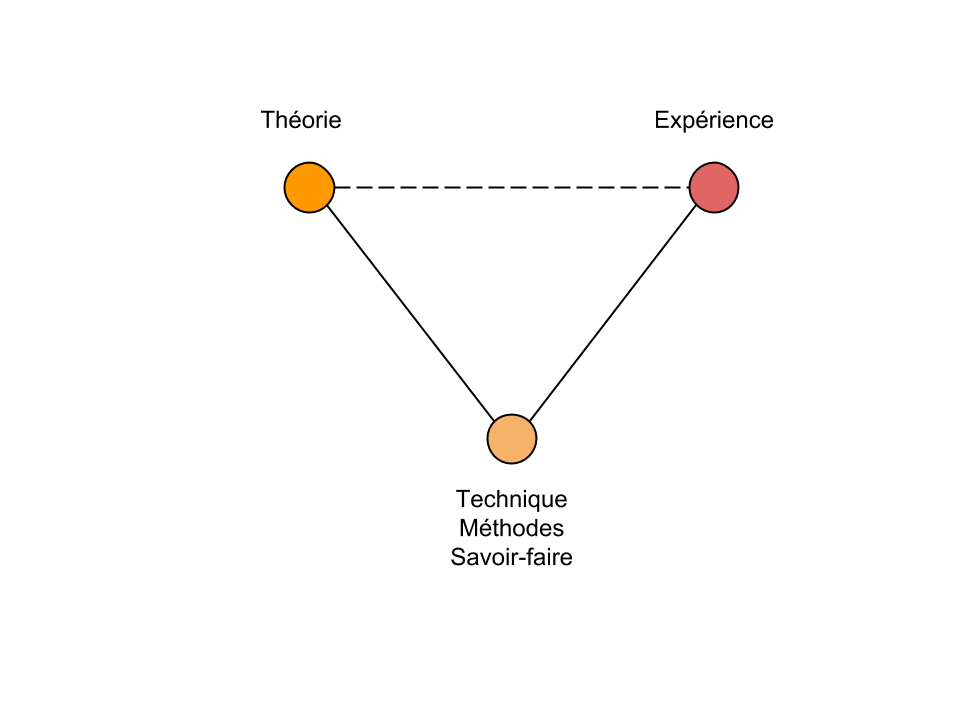
\includegraphics[width=5.0559in,height=3.7894in]{figures/chap3/chapitre3-img1.png}
    \caption[Triptyque des pratiques scientifiques]{Triptyque des pratiques scientifiques}
\end{figure}


En sciences sociales néanmoins, la tension entre la théorie (les concepts), l{\textquoteright}expérience (le terrain) et la méthodologie s{\textquoteright}articule plus rarement autour d{\textquoteright}outillages élaborés. Les \ réflexions sur la méthodologie en sciences sociales portent plus largement sur des argumentations conceptuelles o\`u le langage lui-m\^eme est considéré comme l{\textquoteright}outil premier ou encore de nombreuses réflexions éthiques sur l{\textquoteright}impact des pratiques d{\textquoteright}observation dans le cadre de l{\textquoteright}anthropologie notamment. En France, l{\textquoteright}intér\^et constant porté à l{\textquoteright}utilisation des différentes formes de technologie en sciences humaines s{\textquoteright}est souvent constitué autour de la critique de méthodologies quantitatives très répandues outre atlantique - la statistique en sociologie, l{\textquoteright}étude comportementaliste en psychologie ou le film ethnographique \citep{Becker1996}. Comme le note justement Latour, la qu\^ete de légitimité des Sciences Sociales s{\textquoteright}est souvent traduit par une capacité à se procurer et traiter des données : \textit{{\textquotedblleft}Sociology has been obsessed by the goal of becoming a quantitative science.{\textquotedblright}} \citep{Latour2003}. Pourtant, il serait illusoire de corréler la quantité de données à une quelconque objectivité de la démarche scientifique, tant les démarches et outils nécessaires pour la collecte sont en soi autant de biais importants. La question de la réussite des études utilisant les Big Data semble davantage corrélée à la capacité d{\textquoteright}une approche méthodologique forgée dans un échange interdisciplinaire et des pratiques renouvelées de l{\textquoteright}écriture. La complexité des questions abordées lors du traitement des données, non seulement technologique mais aussi dans les interrogations sur la légitimité de leur existence, leur utilisation et leur provenance \citep{Boyd2011} rendent nécessaire la discussion entre de multiples connaissances. Aujourd{\textquoteright}hui, l{\textquoteright}utilisation de l{\textquoteright}ordinateur conditionne l{\textquoteright}écriture scientifique de l{\textquoteright}étude de terrain, la prise de notes, la rédaction ou la publication et se présente ainsi comme un impératif méthodologique pour la réflexion et le travail en sciences humaines et sociales \citep{Wieviorka2013}. L{\textquoteright}appareillage projeté au centre de la pratique quotidienne du chercheur vient modifier le travail de réflexion sur les phénomènes étudiés et s{\textquoteright}accompagne de multiples contraintes. La prise en main de ce nouvel \textit{{\textquotedblleft}instrument intellectuel{\textquotedblright} }\citep{Guichard2014} passe par une lente alphabétisation aux langages des machines. L{\textquoteright}angoisse latente du {\textquotedblleft}bug{\textquotedblright} n{\textquoteright}est pas apaisée par les rares techniciens présents dans les centres de recherche en sciences humaines, souvent déjà dépassés par la diversité des demandes technologiques. L{\textquoteright}écriture, savoir-faire indispensable de la recherche, possède une nouvelle matérialité dans les disques durs produisant une dépendance accrue aux réseaux d{\textquoteright}ordinateurs. Cette empreinte {\textquotedblleft}digitale{\textquotedblright} laissée par les calculateurs sur les pratiques scientifiques n{\textquoteright}est ni anodine ni révolutionnaire et s{\textquoteright}inscrit dans la longue tradition des cultures de l{\textquoteright}écrit qui déjà bien avant les moines copistes \textit{{\textquotedblleft}combinent les gestes de la main et les opérations de la pensée.{\textquotedblright}} \citep{Jacob2011}  

Tim Berners-Lee, considéré comme l{\textquoteright}inventeur du World Wide Web et du Web Sémantique définit la constitution d{\textquoteright}un réseau mondial des savoirs comme un projet d{\textquoteright}\textit{{\textquotedblleft}ingénierie philosophique{\textquotedblright} }\citep{Halpin2014}. Mi-philosophe mi-ingénieur, le chercheur contribuant à ce réseau de savoir doit donc \^etre en capacité de conna\^itre les protocoles et les langages pour y accéder et s{\textquoteright}y mouvoir aisément. La méthode scientifique s{\textquoteright}écrit notamment avec de nouvelles formulations (fonctions, algorithmes, code...). Les données générées par les usages d{\textquoteright}un nombre croissant de machines communicantes et productrices d{\textquoteright}information, souvent désignées par le concept {\guillemotleft} valise {\guillemotright} de Big Data \citep{Lohr2012} offrent des possibilités nouvelles pour l{\textquoteright}étude en sciences sociales. L{\textquoteright}analyse de ces vastes jeux de données s{\textquoteright}accompagne également de nouveaux impératifs et questionnements sur l{\textquoteright}observation des phénomènes humains qu{\textquoteright}ils représentent. à la fois barrière et opportunité, une difficulté majeure réside dans le discernement nécessaire entre praxis des outils informatiques, fascination pour ces outils et réflexions pertinentes sur la qualité des méthodes employées. Le traitement quantitatif par ordinateur permet d{\textquoteright}extraire de nombreuses connaissances utiles de jeux de données parfois très importants mais n{\textquoteright}assure pas pour autant la qualité des résultats. Une bonne compréhension de la provenance et des méthodes de collection des données est nécessaire afin d{\textquoteright}identifier des algorithmes de traitements intéressants, adaptés et efficaces parmi ceux disponibles \citep{Rajaraman2011}. Les méthodologies d{\textquoteright}exploration et de recherche utilisant le {\textquotedblleft}Big Data{\textquotedblright} comme source nécessitent la mise en {\oe}uvre d{\textquoteright}une ingénierie complexe soutenue par une connaissance des technologies nécessaires à l{\textquoteright}analyse de données. L{\textquoteright}algorithmique, la statistique, l{\textquoteright}informatique mais également la cartographie et le design graphique doivent se conjuguer pour permettre de produire des résultats à la fois intéressants et fiables. Ce travail d{\textquoteright}hypothèses et de vérifications pour l{\textquoteright}analyse de données doit réunir de nombreuses compétences. La définition de la problématique la plus adaptée nécessite une connaissance aig\"ue du terrain et des outils et algorithmes qui seront articulés au sein d{\textquoteright}un système ingénierique parfois très complexe. Le design et la lecture d{\textquoteright}algorithme pour le \textit{{\textquotedblleft}data mining{\textquotedblleft}} sont donc les clés pour le travail du chercheur confronté aux données. Néanmoins, ces algorithmes ne devraient \^etre que la traduction de questions formulées gr\^ace à une connaissance aig\"ue des problématiques du contexte et des objets étudiés - notamment pour identifier les données manquantes. La {\textquotedblleft}science des données{\textquotedblright} promet donc d{\textquoteright}apporter un véritable renouveau des méthodes et des résultats scientifiques, au prix d{\textquoteright}un travail soutenu pour faire face à ces changements d{\textquoteright}habitudes et de langages. Les applications statistiques du {\textquotedblleft}big data{\textquotedblright} permettent aujourd{\textquoteright}hui une fiabilité accrue des prédictions par l{\textquoteright}augmentation du volume des corpus traités \citep{Breiman2001}. Le domaine de l{\textquoteright}intelligence artificielle (AI) a grandement bénéficié de l{\textquoteright}accroissement de la capacité de traitement des données notamment pour la prédiction gr\^ace au techniques dites de \textit{machine learning}. Néanmoins Peter Norvig, directeur de recherche chez Google, reconnait lui-m\^eme : {\textquotedblleft}\textit{We could draw this curve: as we gain more data, how much better does our system get? And the answer is, it{\textquoteright}s still improving---but we are getting to the point where we get less benefit than we did in the past.{\textquotedblright} }\citep{Somers2013}. Comme le note Douglas Hofstadter, un des pairs de l{\textquoteright}Intelligence Artificielle à propos du super-ordinateur qui venait de battre Kasparov aux échecs : \textit{{\textquotedblleft}Okay, Deep Blue plays very good chess---so what? Does that tell you something about how we play chess? No. Does it tell you about how Kasparov envisions, understands a chessboard?{\textquotedblright} }\citep{Somers2013}.  

En effet, ces pratiques méthodologiques doivent réussir à s{\textquoteright}inscrire dans la continuité de l{\textquoteright}historicité et des exigences des disciplines. La portabilité des méthodes et la disponibilité des données sont encore des questions centrales et non-résolues. En sciences sociales notamment, les services de réseaux sociaux en ligne offrent de très larges corpus dont l{\textquoteright}utilisation est régie par les exigences commerciales des sociétés privées qui les détiennent. L{\textquoteright}analyse des données issues de service de réseaux sociaux en ligne est pourtant un champ d{\textquoteright}études en rapide expansion \citep{Nettleton2013}. Pourtant, le débat sur la validité des éclairages apportés par l{\textquoteright}analyse des données issues des services de réseaux reste encore largement ouvert et nous entendons dans ce travail de recherche y contribuer.  


\subsection[Visualisation et espace perceptif pour l{\textquoteright}information]{3.1.3 Visualisation et espace perceptif pour l{\textquoteright}information}

Face à de larges volumes de données, un des grands enjeux est d{\textquoteright}en restituer une forme intelligible afin d{\textquoteright}identifier des tendances ou des motifs particuliers. La visualisation permet de produire une lecture particulière de parties intéressantes et intelligibles d{\textquoteright}un jeu de données \citep{Cairo2013}. Définie comme \textit{{\guillemotleft}~a process that transforms data, information, and knowledge into a form that relies on the human visual system to perceive its embedded information.{\textquotedblright}} \citep{Graffieti2010}, la visualisation introduit la question du design visuel au c{\oe}ur de la problématique d{\textquoteright}analyse \citep{Wesolowsky1992}. La visualisation correspond à une série d{\textquoteright}actions qui résulte dans la production de marqueurs visuels (points, ligne, aires, surface, volume) avec comme étapes la définition de leurs propriétés rétiniennes (couleur, taille, texture, etc.) et leur positionnement dans l{\textquoteright}espace visuel \citep{Card1997}. Dans son travail, Engelhardt \cite{Engelhardt2007} s’attache   à définir les bases d{\textquoteright}une grammaire de la visualisation en commen\c{c}ant par en identifier les formes syntaxiques :  
\begin{enumerate}
\item les objets graphiques montrés (ex. point, flèche, pictogramme, etc.), 
\item l{\textquoteright}espace graphique donnant sens à l{\textquoteright}organisation des objets (ex. systèmes de coordonnnées géographiques, timeline, etc.), 
\item les propriétés graphiques des objets (couleurs, tailles, etc.), 
\item l{\textquoteright}organisation des objets en différentes catégories (ex. cadre, liens, légendes, etc.). 
\end{enumerate}

Ces choix forment une t\^ache importante dont l{\textquoteright}enjeu n{\textquoteright}est pas seulement visuel, mais se joue également dans le champ de la représentation o\`u les objets sont donnés à voir et par là-m\^eme donnés à comprendre. Les travaux sur l{\textquoteright}apparition de la perspective dans la Renaissance italienne ont montré comment l{\textquoteright}espace de la représentation visuelle fait écho aux changements sociétaux profonds de l{\textquoteright}époque \citep{Raynaud2005}. Au-delà d{\textquoteright}une simple technique picturale, les {\oe}uvres des peintres du Quattrecento témoignent de changements profonds dans la perception : l{\textquoteright}espace perceptif se structure désormais autour du sujet et \ de son {\textquotedblleft}point de vue{\textquotedblright} qui construit l{\textquoteright}ensemble de la représentation \citep{Damisch1999}. Empreinte de rationalité, la perspective construit comme au thé\^atre un espace de représentation centré autour du spectateur. En 1639, le mathématicien Desargues modélise les notions intuitives de perspective et d{\textquotesingle}horizon gr\^ace à la géométrie projective qui permet d{\textquoteright}étudier les propriétés inchangées des figures lors de leur projection. Cette géométrie d{\textquoteright}un genre nouveau se structure autour du \textit{plan projectif}, élément topologique qui \textit{{\textquotedblleft}rassemble en une seule surface l{\textquoteright}imagination de tous les points de vue possible{\textquotedblright} }\citep{Petit1999}. En construisant un plan géométrique fondé sur le point de vue, de nouveaux \^etres géométriques aux propriétés étranges voient le jour, dont l{\textquoteright}existence logique force notre représentation classique : la bande de M\"obius ne possède qu{\textquoteright}une seule face et il est impossible de distinguer l{\textquoteright}intérieur de l{\textquoteright}extérieur d{\textquoteright}une bouteille de Klein. Dans ces surfaces dites \textit{unilatères}, le local est traversé en tout point par un tout global. Nous ne pouvons pas traverser puisque nous somme toujours sur la m\^eme face. Ni bord, ni extérieur, ni intérieur, le plan projectif apporte des éléments de réponses conceptuelles aux limites des la représentation dans l{\textquoteright}espace.

Dans le contexte de systèmes et de réseaux complexes, la visualisation de données structure l{\textquoteright}espace perceptif afin de construire une scène à \textit{n }dimensions dont l{\textquoteright}enjeu est la recherche d{\textquoteright}un {\textquotedblleft}point de vue{\textquotedblright} pour l{\textquoteright}étude\textit{. }Alors que la perspective prend pour parti de matérialiser le sujet au centre de la représentation par des points de fuite, la visualisation de données cherche elle à utiliser les objets comme dimensions du champ de la représentation, en structurant souvent l{\textquoteright}espace autour de quantités. Néanmoins, la place du spectateur / utilisateur dans la visualisation reste un des enjeux majeurs encore à explorer. En élaborant sa {\textquotedblleft}méthode graphique{\textquotedblright} , J.E. Marey \citep{Marey1885} utilise la photographie pour créer un nouvel espace de représentation du mouvement et observer des phénomènes jusqu{\textquoteright}ici invisibles. Si la temporalité de l{\textquoteright}écrit ou de la voix est avant linéaire, l{\textquoteright}espace visuel permet de manier le réel pour le décomposer en actes logiques. Charcot cherche dans les images de l{\textquoteright}hystérie des témoignages de la folie et procède à la mise en scène de ses patients dans ce nouvel espace de représentation ouvert par la photographie \citep{DidiHuberman2012}.

La visualisation scientifique se prévaut donc d{\textquoteright}une existence avant tout pratique dont le premier objectif serait de \textit{{\guillemotleft}~to effectively convey information~{\guillemotright}} \citep{Kelleher2011}. Son caractère syncrétique et sa capacité à résumer une large masse d{\textquoteright}information rapidement en font un des plus importants éléments de la publication en science notamment pour sa diffusion et la facilitation d{\textquoteright}accès à une connaissance \citep{Ware2004}. Dans sa sémiologie graphique, Bertin \citep{Bertin1977} distingue deux usages majeurs des graphiques de visualisation : 1) un moyen de communiquer des informations (dans le cas o\`u l{\textquoteright}information a déjà été comprise) 2) un moyen visuel de résoudre des problèmes logiques (quand le graphique est utilisé comme support de lecture et de manipulation d{\textquoteright}informations). Ces deux caractéristiques peuvent coexister dans certaines pièces mais la transition entre les deux nécessite souvent un travail important de restructuration visuelle. Dans le traitement et la visualisation des données \textit{l{\textquoteright}interface }joue un r\^ole primordial. On peut désormais agir sur la deuxième catégorie de Bertin pour mieux explorer le sens \citep{Weissberg2007}. Manovich montre comment l{\textquoteright}interface définie comme \textit{{\textquotedblleft}the ways to represent ({\textquoteleft}format{\textquoteright}) and control the signal.}{\textquotedblright} \citep{Manovich2013}. Ce formatage nouveau de l{\textquoteright}information induit des changements dans la pratique de la lecture qui, toujours selon Manovich, s{\textquoteright}apparenterait davantage à de la reconnaissance de \textit{pattern}, symbolisé par l{\textquoteright}usage de l{\textquoteright}ic\^one et du menu en design d{\textquoteright}interface. Ainsi si l{\textquoteright}interface contraint la lecture, la prise en compte des formes narratives (les \textit{patterns} de Manovich) prend une grande importance quand il s{\textquoteright}agit de concevoir une visualisation d{\textquoteright}information. L{\textquoteright}usage des signes graphiques doit se faire avec une connaissance des usages de l{\textquoteright}interface, afin de recréer la coopération textuelle des r\^oles de lecteur et de designer/auteur nécessaire pour la production un sens \citep{Eco1985}. La \textit{citizen science} ou encore \textit{night science} a fait de l{\textquoteright}interface un paradigme en utilisant la visualisation pour amener un grand nombre de collaborateurs à explorer et analyser de vastes jeux de données en effectuant des t\^aches simples \citep{Silvertown2009}. Le projet \textit{Eyewire} permet à des internautes de contribuer à la classification d{\textquoteright}images du cerveau humain en vue de la réalisation d{\textquoteright}un modèle 3D \citep{Seung2012}. Utilisant des scans de tranches de 1mm réalisés par l{\textquoteright}institut Max Planck, la modélisation 3D d{\textquoteright}un cerveau complet promet une belle contribution pour la découverte des fonctionnements cognitifs. Néanmoins, la t\^ache est colossale et nécessiterait plusieurs années pour une équipe classique de scientifiques. \textit{Eyewire} propose donc une interface web o\`u un simple jeu de coloriage permet d{\textquoteright}identifier les neurones et de contribuer ainsi au dessin du modèle 3D.

Cartes, code ou graphiques, les nouveaux outils numériques participent donc à structurer de nouvelles pratiques de l{\textquoteright}espace numérique gr\^ace à la construction de nouvelles représentations. 

\section[Méthodes et outils d{\textquoteright}analyse des réseaux sociaux]{Méthodes et outils d{\textquoteright}analyse des réseaux sociaux}

Nous allons maintenant regarder comment l{\textquoteright}analyse des données des services de réseaux sociaux en ligne (SNA) peut permettre d{\textquotesingle}interroger les pratiques des technologies numériques pour mieux en comprendre les tenants. 


\subsection[Anatomie d{\textquoteright}un réseau social]{ Anatomie d{\textquoteright}un réseau social}

La représentation des relations sociales sous forme de graphe trouve son origine dans les travaux des psychologues allemands de la \textit{gestalt }durant les années 1920-1930 \citep{Scott1988}\textit{. }S{\textquoteright}inspirant des études sur le cerveau, le psychologue J. L. Moreno s{\textquoteright}applique notamment à comprendre les principes organisationnels holistiques des groupes humains et fonde la sociométrie avec comme objectif la qualification et la quantification des relations sociales \citep{Moreno1938}. Moreno cherche à identifier et isoler des leaders de groupes sociaux définis en étudiant l{\textquoteright}asymétrie ou la réciprocité de leurs choix et fréquentations amicales. Cherchant des moyens de représenter les tendances à l{\textquoteright}auto-organisation qu{\textquoteright}il observe, il cartographie les relations directes et indirectes entre personnes sous forme de \textit{sociogrammes}. Les anthropologues s{\textquoteright}emparent rapidement de ce type d{\textquoteright}outils pour comprendre les formes tribales (Lundberg, 1936) et l{\textquoteright}émergence progressive de la topologie comme domaine important des mathématiques vient définir de nouveaux types de relations entre objets disparates, avec notamment la théorie des graphes qui donne à l{\textquoteright}étude des réseaux ses modèles logiques \citep{Harary1977}. Milgram \citep{Travers1969} voit les relations humaines comme autant de petits mondes (\textit{small-worlds)} connectés entre eux. Granovetter s{\textquoteright}intéresse à l{\textquoteright}importance des relations ténues et lointaines (\textit{weak ties}) dans l{\textquoteright}acquisition d{\textquoteright}informations importantes \citep{Granovetter1973}. L{\textquoteright}influence de la théorie des graphes amène notamment les sociologues à expérimenter de nouveaux modèles venus de la physique ou de la biologie, en proposant de nouvelles pratiques comme celle de la simulation sociale \citep{Epstein1996}. 


La matérialité de l{\textquoteright}image du \textit{graphe} structure la représentation du réseau social. Dans la littérature concernant les réseaux, les notions de graphe et de réseau sont interdépendantes et la théorie des graphes sert notamment de systèmes de notation pour la mise en équation des réseaux \citep{Nettleton2013}. Si cette structure point-ligne semble toutefois rev\^etir une limite de taille pour la description de phénomènes humains (comment en effet réduire les relations humaines à une simple ligne?), elle semble néanmoins aujourd{\textquoteright}hui encore difficile à dépasser.

\begin{figure}
    \centering
    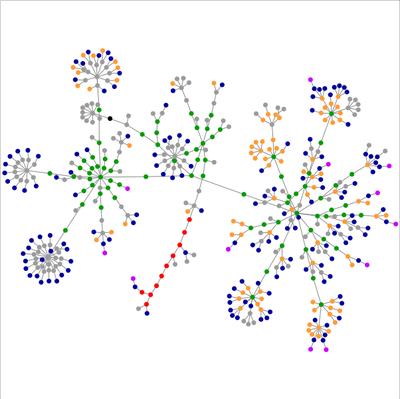
\includegraphics[width=4.178in,height=4.1449in]{figures/chap3/chapitre3-img2.png}
    \caption{Représentation d'un réseau sous forme de graphes.}
\end{figure}


Un réseau considéré comme graphe, noté \textit{G}, se compose d{\textquoteright}un ensemble de nodes ou vertices (les points) et de liens ou edges (les traits). On représente ainsi un graphe sous la notation \textit{G(V,E)} o\`u \textit{V }est l{\textquoteright}ensemble des nodes du réseau et \textit{E} l{\textquoteright}ensemble des liens\textit{ }décrivant leurs relations. \textit{E }décrit les relations entre les nodes qui peuvent \^etre directionnelles (paires de vertices ordonnées) dans le cas d{\textquoteright}un graphe \textit{orienté }ou accompagné de valeurs particulières dans un graphe dit \textit{pondéré. }Les relations ainsi exprimées portent sur un aspect unique, quantifiable et isolable. La prise en compte de facteurs multiples, comme notamment l{\textquoteright}espace physique, le temps, mais également les multiples réseaux de relations qui peuvent exister entre deux acteurs nous amènent à considérer un graphe disposant de multiples couches \textit{(}\textit{multi-layered)} pour décrire l{\textquoteright}ensemble des groupes de relations. Imaginons un graphe de personnes \textit{G (V,E}\textit{\textsubscript{n}}\textit{)} o\`u \textit{V }sont les vertices représentant les personnes et \textit{E}\textsubscript{n} un nombre \textit{n }d{\textquoteright}ensemble de liens\textit{ }décrivant chaque type de relations spécifiques. Le graphe ci-dessous montre un exemple d{\textquoteright}un graphe multi-couche o\`u \textit{E}\textit{\textsubscript{1}} est l{\textquoteright}ensemble des relations amicales, \textit{E}\textit{\textsubscript{2}}\textsubscript{ }les relations de travail et \textit{E}\textit{\textsubscript{3}}\textsubscript{ }les relations familiales.

\begin{figure}
    \centering
    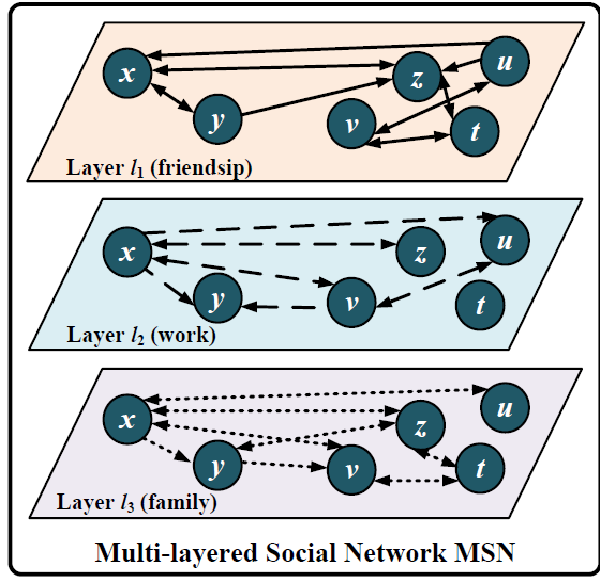
\includegraphics[width=3.8004in,height=3.6894in]{figures/chap3/chapitre3-img3.png}
    \caption [réseau social multi-couches] {Un réseau social multi-couches, d{\textquoteright}après (Brodka\&al., 2013)}
\end{figure}

Nous pouvons ainsi décrire différents jeux de relations entre un jeu d{\textquoteright}acteurs finis, permettant notamment de mieux comprendre les relations entre ses différentes dimensions. Si cette approche résout momentanément la question des \textit{n }dimensions à considérer \citep{Brodka2013} elle augmente également la complexité du graphe et la possibilité d{\textquoteright}erreurs de lecture ou de typage des relations.

Afin de mieux comprendre l{\textquoteright}organisation d{\textquoteright}un réseau, nous disposons de plusieurs mesures~pour décrire les relations et le r\^ole des différents acteurs :

\begin{itemize}
\item \textit{Degree} : (\textit{degré} ou \textit{valence}) mesure le nombre de connections d{\textquoteright}un n{\oe}ud dans un réseau. Cette valeur indique souvent une possibilité, le potentiel d{\textquoteright}un node donné à interagir avec d{\textquoteright}autres.  
\item \textit{Closeness : }(proximité) mesure la facilité d{\textquoteright}un node à se connecter à un autre. Dans un réseau en ligne, on calcule la proximité en estimant la distance la plus courte entre un node et un autre. 
\item \textit{Betweenness} (\textit{centralité}) mesure le degré d{\textquoteright}importance d{\textquoteright}un node dans le réseau en prenant en compte le nombre de nodes dépendant de lui pour
établir une connection entre eux. La centralité représente la capacité à bloquer ou laisser filtrer l{\textquoteright}accès à certaines parties du réseau. Dans une entreprise par exemple, la secrétaire du CEO a par exemple une très haute centralité.
\end{itemize}

En observant ces différentes mesures, nous pouvons définir différentes structures types pour chaque réseau. La distribution des degrés dans le graphe permet notamment de comprendre les modèles qui régissent les connexions entre les nodes. L{\textquoteright}exemple le plus simple est le \textit{random network, }réseau o\`u les acteurs sont connectés de manière entièrement aléatoire. Un réseau dont le degré de distribution correspond à une loi de puissance est appelé \textit{scale-free network. }Un réseau dont seulement quelques nodes possèdent une centralité élevée et dont la structure d{\textquoteright}ensemble est faite de groupes ou \textit{clusters} interconnectés et appelé un \textit{small-world network}.

\begin{figure}
    \centering
    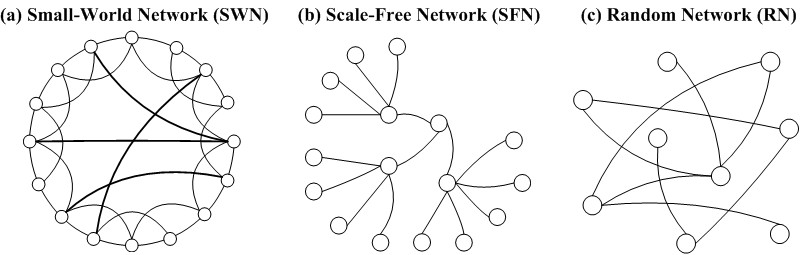
\includegraphics[width=6.3449in,height=2.0224in]{figures/chap3/chapitre3-img4.jpg}
    \caption{Types communs de réseaux}
\end{figure}

Les services de réseaux sociaux en ligne sont structurés en \textit{small-worlds}. Dans une étude analysant de larges corpus issus de différents services de réseaux sociaux en ligne, Kumar \& al. \citep{Kumar2006} ont montré que ces communautés possèdent toutes une structure et une évolution similaire. Les inscrits de chaque service se répartissent autour de trois grands groupes : \textit{singletons} (membres isolés, inactifs), \textit{giant component} (la majorité des utilisateurs actifs) et \textit{middle region} (des communautés isolées qui interagissent entre elles mais pas avec le reste du réseau). D{\textquoteright}après les auteurs, il existe très peu de chances que deux communautés isolées m\^eme très similaires se rencontrent dans ce type de réseau, car l{\textquoteright}entropie de la structure \textit{small-world }se renforce avec le temps en se fragmentant davantage. Une des raisons principales est que ces communautés isolées suivent souvent un modèle en \textit{étoile, }c{\textquoteright}est à dire qu{\textquoteright}elles sont construites autour d{\textquoteright}un individu central charismatique. éventuellement, il leur arrive de rejoindre la masse du \textit{giant component} mais elles en deviennent difficilement des acteurs majeurs et restent en périphérie. Dans un réseau social de type small-world comme les OSNS, les acteurs les plus influents sont ceux qui sont capables de 1) renforcer les liens dans un cluster (\textit{closure)} et 2) développer les connections faibles entre des clusters (\textit{brokerage)} (Burt, Centola, \& Kahl, 2008). Ce {\textquotedblleft}capital social{\textquotedblright} est inscrit dans la structure du réseau social lui-m\^eme \citep{Lin1999} et n{\textquoteright}a pas de relations avec le degré du node (son nombre de connections) \citep{Cha2010}. L{\textquoteright}individu le plus puissant d{\textquoteright}un réseau est donc celui possédant le plus grand nombre de connections \textit{potentielles, }proches et facilement accessibles et qui bénéficie d{\textquoteright}une place privilégiée pour bloquer ou autoriser l{\textquoteright}accès aux autres parties du réseau. L{\textquoteright}analyse organisationnelle a notamment montré l{\textquoteright}importance capitale des secrétaires pour le maintien d{\textquoteright}une bonne circulation des informations dans le réseau de l{\textquoteright}entreprise ou la nécessité d{\textquoteright}un nombre très faible de connections directes pour les acteurs importants de réseaux terroristes ou mafieux \citep{Russel2011}.


\subsection[Diffusion des discours dans les réseaux sociaux]{Diffusion des discours dans les réseaux sociaux}

L{\textquoteright}analyse de réseau social permet de comprendre la structure d{\textquoteright}un moment du réseau. En effet, les connections entre différents acteurs sont sans cesse en mouvement et l{\textquoteright}information en circulant vient modifier l{\textquoteright}activité du réseau et bien souvent sa structure m\^eme. Notre étude porte sur la diffusion de mèmes au sein du réseau social chinois Sina Weibo et s{\textquoteright}inscrit ainsi dans la continuité des travaux s{\textquoteright}intéressant aux rapports entre diffusion et technologies. Néanmoins, le champ de la diffusion de l{\textquoteright}innovation, objet traditionnel de la géographie, s{\textquoteright}est largement constitué autour des problématiques technologiques et organisationnelles liées à la situation spatiale du lieu et ses équipements \citep{Crevoisier2004}. Les études urbaines ont notamment montré comment la réalité économique et géographique présidait à la constitution des savoirs nécessaires à la diffusion de l{\textquoteright}innovation technologique \citep{Howells2002}. Cette vision doit \^etre modérée par une considération plus importante des modalités d{\textquoteright}appropriation des technologies comme pratiques propres aux territoires \citep{Fernandez2010}. Plus largement, les études sur la diffusion sont dominées par l{\textquoteright}analogie du virus comme modèle de propagation des messages, comportements et idées. Depuis la fin du XIXe siècle \citep{LeBon1895}, ce modèle est prépondérant dans les recherches autour de la diffusion d{\textquoteright}information en ligne \citep{Goel2012} Les membres de groupes dans un réseau seraient \textit{exposés }à un message ou une idée avant d{\textquoteright}\^etre \textit{infectés, }devenant alors porteur puis agent de sa diffusion. Ainsi, en considérant la position d{\textquoteright}un individu au sein du réseau de diffusion, il serait possible de définir un \textit{{\textquotedblleft}}\textit{degré d{\textquoteright}infection{\textquotedblright}} \citep{Cheng2013} et d{\textquoteright}anticiper la diffusion selon une \textit{{\guillemotleft}~probabilité immune~{\guillemotright} }qui\textit{ }déciderait de la \textit{{\guillemotleft}~qualité infectieuse~{\guillemotright} }de l{\textquoteright}objet diffusé ou de la \textit{{\guillemotleft}~possibilité de }\textit{rétablissement~{\guillemotright} }du sujet infecté \citep{Wang2011}. Cette analogie du viral propose une vision mécaniste qui fait peu de cas des facteurs contextuels ou psychologiques et ignorent ainsi les processus de décisions individuels en jeu \citep{Jackson2010}. Pourtant, nous savons notamment que le choix des mots ou la situation des personnes diffusant un message sont des facteurs décisifs et structurant des processus d{\textquoteright}adoption des messages en ligne \citep{Conover2013}.  En s{\textquoteright}intéressant à la diffusion géographique de mots dans les réseaux sociaux, Eisenstein \& al. \citep{Eisenstein2012} observe que leur diffusion se limite à un domaine géographiquement bien défini, dépendant de facteurs culturels et démographiques. Par exemple, les villes ayant d{\textquoteright}importantes communautés afro-américaines ont davantage de chances d{\textquoteright}adopter un m\^eme mot que d{\textquoteright}autres parfois plus proches géographiquement. Cette question est au centre des études de marketing qui s{\textquoteright}interrogent notamment sur l{\textquoteright}adoption de nouvelles marques ou de slogans. Afin de déterminer statistiquement les possibilités d{\textquoteright}adoption de produits et prévoir la pénétration dans un marché précis, la modélisation mathématique des effets de réseaux dans la diffusion est souvent utilisé \citep{Bass1994}. Ici, l{\textquoteright}analyse des données des réseaux sociaux est un grand enjeu pour la prospective économique et l{\textquoteright}application de ces modèles mathématiques aux données utilisateurs permettant de considérer des segments précis de marché. Le marketing politique fait lui aussi grand cas de l{\textquoteright}analyse de réseaux sociaux pour comprendre et orienter les discussions. La campagne de réélection d{\textquoteright}Obama aux USA en 2012 a fait un usage extensif de l{\textquoteright}analyse de données des réseaux sociaux pour identifier, déterminer et cibler des groupes sociaux particuliers gr\^ace au travail d{\textquoteright}une vaste équipe d{\textquoteright}ingénieurs et de \textit{{\textquotedblleft}data scientists{\textquotedblright}}\footnote{ \textit{{\textquotedblleft}Harper Reed, the chief technology officer for the Obama re-election campaign, who heads a team described as {\textquotedblleft}100 data scientists, developers, engineers, analysts, and old-school hackers [that] have been transforming the way politicians acquire data---and what they do with it.{\textquotedblright}, }from \ The Blaze \url{http://www.theblaze.com/stories/2012/10/03/very-creepy-details-of-obama-campaigns-voter-data-mining-effort/} consulté le 12 Mars 2014 à 14:50 GMT+1}. 

Une des grandes interrogations dans ce domaine est évidemment les r\^oles joués par les différents acteurs du processus de diffusion - et la manière de les identifier. Les études concernant les leaders d{\textquoteright}opinion, traditionnelles en sciences de la communication \citep{Katz1955} trouvent une continuité directe dans l{\textquoteright}étude des réseaux sociaux en ligne avec le domaine florissant des recherches sur l{\textquoteright}identification des \textit{influenceurs} \citep{Bakshy2011, Leavitt2009}. L{\textquoteright}analyse quantitative permet notamment de mieux comprendre l{\textquoteright}influence réelle des acteurs dans le réseau gr\^ace à l{\textquoteright}étude de leurs comportements. Le concept d{\textquoteright}influence sur les réseaux sociaux rev\^et en réalité des formes très variables et procède notamment d{\textquoteright}une légitimité construite autour de sujets précis par \ des personnes spécialisées devenues référentes \citep{Cha2010}. D{\textquoteright}autres {\textquotedblleft}influenceurs{\textquotedblright} possèdent une grande capacité d{\textquoteright}amplification pouvant par exemple initier le développement d{\textquoteright}une \textit{{\textquotedblleft}masse critique{\textquotedblright} }autour d{\textquoteright}une information\textit{, }définie classiquement comme le seuil d{\textquoteright}adoption à partir duquel la diffusion devient pérenne parmi une foule d{\textquoteright}acteurs \citep{Oliver2001}. L{\textquoteright}image quantitative d{\textquoteright}une {\textquotedblleft}masse{\textquotedblright} uniforme et actionnable dans le réseau est néanmoins remise en question par l{\textquoteright}étude de données dont l{\textquoteright}analyse montre que les relations entre différents acteurs du réseau sont à considérer qualitativement en termes de relations de pouvoirs \citep{Steyer2006}\textit{. }Les dynamiques d{\textquoteright}échanges ne répondent en effet pas tant à une relation pré-existente dans le réseau qu{\textquoteright}à un ensemble de situations o\`u les acteurs adoptent des comportements et des réactions particulières. La diffusion peut ainsi se comprendre comme une pratique du \textit{bouche-à-oreille} éminemment contextuelle, o\`u certains acteurs sont plus ou moins influents dans telle ou telle situation ou sur tel et tel sujet. Le temps joue néanmoins un r\^ole déterminant puisqu{\textquoteright}en considérant des séries de résultats o\`u des acteurs se c\^otoient durant plusieurs années, il est souvent difficile d{\textquoteright}identifier quel acteur influence l{\textquoteright}autre \citep{Aral2009}. 

\subsection[Méthodes d{\textquoteright}analyse de données des réseaux sociaux en ligne]{3.2.3. Méthodes d{\textquoteright}analyse de données des réseaux sociaux en ligne}

Après moins d{\textquoteright}un siècle d{\textquoteright}existence, l{\textquoteright}analyse de réseaux sociaux sous forme de graphes a donc connu une rapide évolution et une diversification dans de nombreux domaines de recherche. Les services de réseaux sociaux en ligne offrent notamment la possibilité d{\textquoteright}obtenir des données sur les comportements de groupes sociaux en très vaste quantité. Véritable vivier d{\textquoteright}études, ce champ de recherche en pleine expansion trouve ses origines dans des disciplines diverses qui poursuivent souvent des objectifs et des méthodes très différentes. Le tableau infra présente quelques-unes des méthodes d{\textquoteright}analyse de données définies selon leurs domaines d{\textquoteright}application. Ces méthodes coexistent souvent lors d{\textquoteright}études utilisant le \textit{data mining} ; nous présentons ici des exemples qui permettront ensuite de mieux situer nos perspectives de recherche~dans ce paysage de pratiques.

\begin{landscape}    
    \begin{spacing}{1} % line spacing

    \begin{ltabulary}{L| L J L J}
        &
        \textbf{Courant d{\textquoteright}analyse} &
        \textbf{Méthodologie} &
        \textbf{Exemples d{\textquoteright}usages et applications} &
        \textbf{Auteurs \& Publications de référence} \endhead
        
        \hline \\ [-0.5ex]

        1 &
        Graphes sociaux de groupe définis (cartographie de réseau fini) &
        En partant d{\textquoteright}un échantillon fini et déterminé au préalable, on effectue une carte des relations entre les différents acteurs du réseau.  &
        Cartographier les connections d{\textquoteright}après un profil sur un service de réseau social en ligne  &
        Cette pratique est l{\textquoteright}origine de la sociométrie (Moreno \& Jennings, 1938) et de l{\textquoteright}étude des relatons sociales en tant que réseaux.
        \\
        \hline \\ [-0.5ex]

        2 &
        Découverte de groupes par critères (communautés) &
        Cette méthode permet de réaliser un échantillonnage
        d{\textquoteright}un réseau social à partir d{\textquoteright}un
        ensemble de profils existants appelés \textit{seeds}. Un logiciel
        (appelé \textit{crawler}) va rechercher et collecter les profils
        similaires aux \textit{seeds} selon des critères définis :
        similarité, différence, profondeur, etc. &
        Identifier des communautés d{\textquoteright}après un type
        d{\textquoteright}utilisateur témoin

        Trouver des profils d{\textquoteright}utilisateurs similaires
        d{\textquoteright}après des profils existants &

        Hérité de la tradition de l{\textquoteright}échantillonnage
        \textit{{\textquotedblleft}boule de neige{\textquotedblright}} en
        statistiques \citep{Rothenberg1995}, les algorithmes de \textit{crawling}
        sont nombreux et il n{\textquoteright}existe pas de véritable
        consensus sur leur utilisation \citep{Gjoka2011}
        \\
        \hline \\ [-0.5ex]

        3 &
        Analyse sémantique des conversations (analyse de contenu)
         &
        En utilisant une masse textuelle de posts, un système est chargé
        d{\textquoteright}extraire et de classifier les mots et sujets
        discutés. Ce type de système se fonde sur l{\textquoteright}analyse
        naturelle de langage (NLP) et parfois sur l{\textquoteright}analyse
        structurelle des conversations \citep{Karandikar2010}.
         &
        Détection de tendances dans les conversations, Reconnaissance des
        entités dans un texte~(\textit{semantic tagging}) : noms de lieu,
        personnes, etc. &
        A mi-chemin entre linguistique et informatique \citep{Russel2011}, ce champ
        est un des grands enjeux actuels du Big Data \citep{Nettleton2013} avec
        notamment l{\textquoteright}analyse des sentiments (Liu \& Zhang, 2012)
        \\
        \hline \\ [-0.5ex]
        4 &
        Analyse de la diffusion 

        (évolution des \ relations d{\textquoteright}après une conversation)
        &
        D{\textquoteright}après une masse de posts extraites selon des
        critères précis (souvent un mot-clé ou \textit{hashtag}), il
        s{\textquoteright}agit ici de retracer les dynamiques relationnelles
        qui entourent ou suscitent la conversation en recréant le graphe
        social entourant la discussion et son évolution.  &
        Analyse d{\textquoteright}une campagne de marketing viral, Détection de communautés autour d{\textquoteright}un sujet précis, Détection d{\textquoteright}influenceurs \citep{Cha2010}

        R\^oles et partitionnement des acteurs de la diffusion \citep{Kwak2010b} &
        Le modèle classique du \textit{word-of-mouth }\citep{Steyer2006} et l{\textquoteright}approche
        épidémiologique \citep{Wang2011} sont souvent utilisés
        dans l{\textquoteright}analyse de la diffusion de contenus en ligne \citep{Cheng2013}.
        \\
        \hline \\ [-0.5ex]

        5 &
        Analyse comportementale et agents de diffusion (classifications et
        mesures)

        ~
         &
        Ici on étudie l{\textquoteright}activité d{\textquoteright}un ou
        plusieurs agents en analysant leur comportement dans le réseau
        (volume d{\textquoteright}activité, fréquence, etc.) souvent pour
        définir des critères et mesures qui permettent de classifier par
        type ou d{\textquoteright}anticiper les actions d{\textquoteright}un
        acteur du réseau. &
        Détection d{\textquoteright}influenceurs

        Mesures de la probabilité de diffusion \citep{Anagnostopoulos2012}

        Typologie des utilisateurs par comportement

        Effet psychologique des signaux sur un utilisateur &
        Présentes notamment dans le champ du marketing \citep{Leskovec2005} et de la politique \citep{Lotan2011}, 

        ce type d{\textquoteright}analyse cherche à comprendre et retracer les
        processus parfois psychologiques \citep{Robins2013} de prise de décisions
        individuelle.
        \\
        \hline \\ [-0.5ex]
        6 &
        Analyse contextuelle et géographique  &
        Ce type d{\textquoteright}analyse cherche à mettre en perspective des
        facteurs extérieurs au réseau afin d{\textquoteright}en comprendre
        l{\textquoteright}influence et les effets. Entre sciences sociales et
        informatique, ce type d{\textquoteright}étude porte souvent sur
        l{\textquoteright}usage du réseau plus que sur sa structure ou son
        évolution \citep{Torrens2010,Leetaru2013} &
        Approche sociologique des usages

        Mesures d{\textquoteright}impact \ géographique (node locality,
        geographic clustering coeficient) &
        L{\textquoteright}approche contextuelle dans l{\textquoteright}analyse
        de réseaux restent encore un champ à développer \ \citep{Adams2012}, notamment dans la considération de facteurs
        géographiques \citep{Graham1998, Onnela2011}, culturels \citep{Gallagher2013} ou de langage.
        \\
        \hline \\ [-0.5ex]
        7 &
        Simulation sociale &
        Afin de comprendre les dynamiques en l{\textquoteright}absence de
        données ou pour anticiper une situation à venir, il est possible de
        modéliser un environnement virtuel o\`u les comportements des acteurs
        sont simulés \citep{Macy2002}  &
        Prévision de tendances d{\textquoteright}après des données
        existantes

        Analyse de faits dont les données sont manquantes ou incomplètes &
        La découverte de méthodes de modélisation du contexte de
        l{\textquoteright}univers de simulation \citep{Ronald2012} est un des grands enjeux o\`u
        l{\textquoteright}apport de méthodes ethnographiques de terrain peut
        \^etre crucial \citep{Tubaro2010}\\
        
        % \caption[Tableau récapitulatif de méthodes d{\textquoteright}analyse de données de réseaux sociaux en ligne.]{Tableau récapitulatif de méthodes d{\textquoteright}analyse de données de réseaux sociaux en ligne.}
    \end{ltabulary}
    \end{spacing} % line spacing
\end{landscape}

Notre recherche choisit donc de s{\textquoteright}appuyer sur une étude de cas spécifique de Sina Weibo reprenant les éléments méthodologiques de l{\textquoteright}étude du graphe social de la diffusion entourant les conversations (Fig. 1-4) et l{\textquoteright}analyse sémantique des sujets dominants et sous-jacents aux conversations (Fig. 1-3). également, nous souhaitons amener une plus forte contextualisation des usages (Fig. 1-6) en prenant en compte notamment les relations entre les dimensions sémantique et conversationnelles, mais aussi géographique de l{\textquoteright}existence des conversations. L{\textquoteright}approche de l{\textquoteright}étude des données des SNS par les géographes notamment s{\textquoteright}est jusqu{\textquoteright}ici largement focalisée sur l{\textquoteright}analyse des \textit{geotag} et des cartes en ligne comme principale approche méthodologique \citep{Graham2011, Poorthuis2013}, réduisant considérablement les possibilités d{\textquoteright}étude des données de réseaux sociaux en ligne \citep{Crampton2013}. Nous souhaitons ici mettre en perspective ces différentes dimensions afin d{\textquoteright}enrichir le modèle d{\textquoteright}étude. En effet l{\textquoteright}analyse de la diffusion utilise principalement les graphes des réseaux de diffusion mettant en scène les utilisateurs et leurs interactions en ligne. Loin d{\textquoteright}\^etre inintéressant, ce type de schéma est néanmoins très réducteur car il se fonde sur un modèle communicationel très primaire \textit{{\textquotedblleft}émetteur-récepteur{\textquotedblright} }dont on conna\^it les limites. Les travaux de Jacobson ont notamment permis d{\textquoteright}étoffer ce modèle en considérant les différents aspects fonctionels des actes de communication.


\begin{figure}
    \centering

    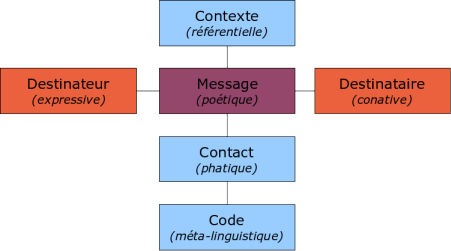
\includegraphics[width=4.6894in,height=2.6114in]{figures/chap3/chapitre3-img5.png}

    \caption[Modèle de Jakobson]{ Le modèle de Jakobson présente différents aspects des actes de communication que nous pouvons chercher à adapter dans le contexte des échanges en ligne.}

\end{figure}

Ainsi, en nous basant sur les modèles des théories de la communication, nous pouvons peut-\^etre améliorer les modèles méthodologiques d{\textquoteright}analyse. Nous proposons ici la notion de \textit{topogramme }comme modèle pour comprendre les motifs de diffusion des mèmes, considérés comme \textit{topos} ou \textit{lieux communs. }Le topogramme, en tant que représentation graphique des différentes dimensions et dynamiques lisibles dans les données nous permet donc d{\textquoteright}approcher un travail \ d{\textquoteright}observation précise de la diffusion des mèmes, voire par la suite de classification des actes de communication en ligne. Afin de prendre en compte, les différents aspects de la communication, il nous faut donc effectuer une analyse à plusieurs niveaux (multi-layers), regroupant un ensemble de réseaux à la fois sémantique, conversationnel et géographique.


\section{Méthodologie choisie et schemes d{\textquoteright}analyse retenus}

\subsection[Constitution et collection d{\textquoteright}un corpus de données]{Constitution et collection d{\textquoteright}un corpus de données}

Afin de poursuivre notre étude, nous allons donc procéder à l{\textquoteright}analyse de données issues de services de réseaux sociaux en ligne. La plupart des services de réseaux sociaux en ligne offrent un large accès car il s{\textquoteright}agit souvent de la fondation de leurs modèles d{\textquoteright}affaires basés sur la valorisation et la revente de ces données pour le marketing ciblé \citep{Ko2010}. Pour entrer en contact avec la base de données, les SNS mettent à disposition une API (\textit{Application Programming Interface}) qui permet à un programme ou une autre application web de se connecter au service pour demander et obtenir des données. L{\textquoteright}API est donc la première source d{\textquoteright}obtention de données depuis les SNS. Néanmoins, les données des réseaux sociaux sont soumises à d{\textquoteright}importants enjeux et contraintes tant commerciales, éthiques que politiques dans le cas de la Chine notamment. Les conditions d{\textquoteright}utilisations techniques et légales (\textit{Terms of Uses) }de ces données sont également soumises à des changements fréquents, étroitement liés à l{\textquoteright}évolution commerciale et technologique de compagnies souvent très jeunes. Nous avons établi une liste des limitations et écueils pouvant \^etre rencontrés lors de l{\textquoteright}extraction et de l{\textquoteright}analyse de données des SNS :

\begin{description}
    
    \item[Compatibilité] Une solution technologique devient facilement caduque lors de l{\textquoteright}évolution d{\textquoteright}une API (ex. Twitter APi v1.0 n{\textquoteright}existe plus, ainsi le code doit \^etre réécrit pour la version 1.1).  
    
    \item [Disponibilité] : Chaque API répond à des formats et critères précis et possède ses propres limitations. Pour accéder à l{\textquoteright}API du moteur de recherche de Sina Weibo, il faut s{\textquoteright}identifier auprès de la compagnie gr\^ace à une carte d{\textquoteright}identité et des paiements par requ\^ete sont exigés.

    \item[Limitations d{\textquoteright}usage] : Afin de limiter le trafic et conserver le contr\^ole sur les données distribuées, les SNS mettent en place des limitations d{\textquoteright}accès à leurs serveurs, notamment : limitation du nombre de requ\^etes par heure, limitation du nombre de requ\^etes par machine (basée sur l{\textquoteright}adresse IP), limitation du nombre d{\textquoteright}utilisateurs connectés. Ainsi, Twitter limite à 150 requ\^etes API par heure pour un compte non identifié, pouvant augmenter jusqu{\textquoteright}à 500 après authentification. Les données datant de plus de 7 jours sont payantes, reflétant la valeur d{\textquoteright}un accès en {\textquotedblleft}temps-réel{\textquotedblright} aux données.
    
    \item[Légalité ] Les données sont soumises aux conditions de propriété décrites légalement par la firme qui les publient \citep{Clifton2006}. Ces conditions sont susceptibles de changer. Ainsi, Twitter a exigé en 2012 le retrait a posteriori de nombreux jeux de données publiés par des chercheurs depuis plusieurs années parfois \citep{McCreadie2012}. Actuellement, Twitter précise notamment dans ses \textit{Terms of Use: {\textquotedblleft}You may not resyndicate or share Twitter content, including datasets of Tweet text and follow relationships{\textquotedblright} }\footnote{ Terms of use de Twitter, \url{https://dev.twitter.com/terms/api-terms}, consulté le 12 Mars 2013 à 17h08}.
    
    \item[Ethique] Vous pouvez extraire depuis une API des profils d{\textquoteright}utilisateurs contenant les informations qu{\textquoteright}ils ont auparavant publié en ligne (Felt \& Evans,  2008). En exposant les données personnelles des utilisateurs, le chercheur est responsable de l{\textquoteright}usage qu{\textquoteright}il fait des données \citep{Rieder2005}  
\end{description}

Afin d{\textquoteright}obtenir des données et de contourner les limitations de l{\textquoteright}API, la pratique dite du \textit{{\textquotedblleft}scraping{\textquotedblright} }permet d{\textquoteright}obtenir des données à l{\textquoteright}aide d{\textquoteright}un robot qui lit et sauvegarde des parties ou l{\textquoteright}intégralité de pages web. Les moteurs de recherche utilisent notamment cette technique pour l{\textquoteright}indexation des pages. Ce type de pratiques est également soumis à des limitations par les services web (blocage de l{\textquoteright}IP source) et se situe à la limite de la légalité,voire est explicitement interdite dans le cas de certains SNS \citep{Petschulat2010}.

Un programme appelé \textit{spider }ou \textit{crawler} est chargé d{\textquoteright}effectuer des requ\^etes régulières à l{\textquoteright}API afin d{\textquoteright}obtenir et collecter les informations obtenues dans une base de données. Plusieurs approches existent dans les techniques échantillonnage de réseau social. La première, fondée sur des mots-clés extraits les posts contenant des mots ou des hashtags particuliers. La seconde utilise l{\textquoteright}échantillonnage de graphe, collectant au fil des liens les conversations ou profils des utilisateurs. Classique des études statistiques, cet échantillonage dit \textit{boule de neige {\textquotedblleft}élargit l{\textquoteright}échantillon en partant d{\textquoteright}un node original pour s{\textquoteright}éloigner vers ses voisins{\textquotedblright}} \citep{Rothenberg1995}. Ici, deux grandes catégories s{\textquoteright}opposent : les techniques traversales o\`u les nodes sont classifiés après avoir été visités et les {\textquotedblleft}walk{\textquotedblright} aléatoires o\`u l{\textquoteright}extension du graphe visité se fait de manière aléatoire \citep{Gjoka2011}.

Au cours du travail préparatoire de cette recherche, nous avons tout d{\textquoteright}abord expérimenté plusieurs algorithmes et outils de collection de données afin d{\textquoteright}en comparer les résultats. Une première approche d{\textquoteright}extraction par utilisateurs a été infructueuse car la sélection du groupe source (\textit{seeds}) ne permettait pas d{\textquoteright}obtenir des résultats cohérents\footnote{ Code disponible : \url{https://github.com/sharismlab/Pyweibo}, consulté le 14 Mars à 5h32}. Par la suite, une autre approche de collecte de données via le développement d{\textquoteright}un plug-in pour le navigateur Google Chrome\footnote{ Code disponible : \url{https://github.com/sharismlab/battlefield}, consulté le 14 Mars à 5h12\par } nous a permis de tester et d{\textquoteright}apercevoir les limites de la collection de données par mots-clés. Cette étape nous a également montré l{\textquoteright}intér\^et que peut présenter une approche collaborative de la collection de données ou de seeds par un système de {\textquotedblleft}curation{\textquotedblright} collaboratifs afin d{\textquoteright}obtenir des éléments précis de contenus et de réduire la masse de données inutiles qui pollue souvent les jeux de données \citep{Ding2013}. Après de multiples tests et comparaisons d{\textquoteright}outils et de librairies, plusieurs difficultés majeures limitaient l{\textquoteright}obtention d{\textquoteright}une quantité de données suffisantes, notamment la nécessité de ressources assez importantes (en terme de développement et de disponibilité des machines), un temps d{\textquoteright}acquisition parfois très long et l{\textquoteright}exigence d{\textquoteright}une veille constante sur les SNS pour identifier un mème au bon moment (les tweets de Sina Weibo devenant indisponibles via l{\textquoteright}API au-delà de 7 jours). La première limite se situe bien s\^ur dans la capacité d{\textquoteright}une personne seule à mener à bien cette large t\^ache. Nous avons donc choisi de considérer les jeux de données collectés sur Sina Weibo disponibles sur l{\textquoteright}Internet. Une fois écartés les nombreux jeux tronqués, modifiés ou incomplets, nous avons pu obtenir plusieurs jeux de données provenant de recherches préalables dans le domaine particulier de l{\textquoteright}échantillonnage \citep{Ding2013} ou ayant servi de bases à des études précédentes \citep{Gao2012}. Finalement, nous avons identifié le jeu de données constitué lors du projet \textit{Weiboscope }de l{\textquoteright}Université de Hong Kong comme répondant à nos besoins en termes de dimensions (temps, nombre d{\textquoteright}utilisateurs observés), taille (nombre de tweets) et contenus (géo-localisation, présence des tweets censurés).


Notre travail d{\textquoteright}analyse s{\textquoteright}appuie donc sur ce jeu de données collecté sur le service de microblog Sina Weibo par le \textit{Journalism and Media Studies Centre} (JMSC) de l{\textquoteright}Université de Hong Kong lors de son projet \textit{Weiboscope}. Téléchargeable ouvertement, la publication de ce jeu de données a pour objectif de \textit{{\textquotedblleft}enables academic use of the data for better understanding of the social }\textit{media in China and making the Chinese media system more transparent.{\textquotedblright}}\footnote{ Le jeu de données Weiboscope est disponible à l{\textquoteright}adresse : \url{http://147.8.142.179/datazip/}, consulté le 14 Mars à 17h21 }\textit{ }Il s{\textquoteright}agit d{\textquoteright}un échantillonnage aléatoire de messages \textit{(random sampling)} effectué quotidiennement durant toute l{\textquoteright}année 2012 sur un panel d{\textquoteright}environ 350 000 utilisateurs ayant au moins 1000 followers \citep{Fu2013}. La totalité du jeu de données comprend 226,841,122 messages répartis sur 52 semaines, dont des messages ayant été supprimés par les utilisateurs eux-m\^emes ou par les administrateurs de Sina Weibo eux-m\^emes - parfois sur ordre du gouvernement chinois (\textit{ibid}, 2013).

\begin{table}[ht]
    \centering
    \small
    \begin{tabulary}{\textwidth}{c|C} 
        \toprule
        \textbf{Désignation}
        & \textbf{Description} \\
        \hline \\[-1.5ex]

        mid  &
        Unique pseudo message ID\\[2ex]
        retweeted\_status\_mid  &
        Pseudo message ID of the original message (Only available if the row of
        interest is a retweet)\\[2ex]
        Uid &
        Pseudo user ID\\[2ex]
        retweeted\_uid &
        Pseudo user ID of the original poster (Only available if the row of
        interest is a retweet)\\[2ex]
        Source &
        The application name of the client program\\[2ex]
        Image &
        With image? (1= Yes, 0=No)\\[2ex]
        text  &
        body of the message. Any address handle (@xxxx:) is replaced by either
        the pseudo user ID or ukn (uknown)\\[2ex]
        geo &
        GIS information. Please refer to the Sina Weibo API documentation:
        \url{http://goo.gl/Um8SS}\\[2ex]
        created\_at &
        Original posting time\\[2ex]
        deleted\_last\_seen &
        The last seen time before this message was missing from the user
        timeline\\[2ex]
        permission\_denied  &
        {\textquotesingle}permission denied{\textquotesingle} status is marked
        when the message was found missing in the timeline and the API return
        message was {\textquotesingle}permission denied{\textquotesingle} - See
        details in (Fu, Chan, Chau 2013)\\[2ex]
    \end{tabulary}
    \caption[Modèle de messages pour le jeu de données Weiboscope]{Modèle de messages pour le jeu de données Weiboscope}
\end{table}

Ce jeu de données a été mis à disposition sous une forme anonymisée o\`u les identifiants des messages et des utilisateurs ont été remplacés par des pseudo-identifiants. La collection des données a été effectuée sur une série d{\textquoteright}utilisateurs (génération aléatoire d{\textquoteright}identifiants dont l{\textquoteright}existence est ensuite validée) pour donner \textit{{\textquotedblleft}une image représentative des usages et utilisateurs de Sina Weibo (...) dont les études auparavant limitée à des analyses non-aléatoire (...) se cantonnaient aux utilisateurs les plus populaires{\textquotedblright} }\citep{Fu2013}. Ainsi, plut\^ot que de considérer uniquement les {\textquotedblleft}stars{\textquotedblright} de Sina Weibo, cet échantillon s{\textquoteright}attache à refléter également les pratiques des utilisateurs {\textquotedblleft}lambda{\textquotedblright}. Ce jeu de données a déjà été partiellement étudié dans le but de comprendre la démographie des utilisateurs de Sina Weibo, leurs activités et les comportements pouvant permettre de prédire les réactions notamment de censure \citep{Fu2013}. La démographie des utilisateurs se composent de 55\% d{\textquoteright}hommes habitant principalement dans les grandes villes de Chine (Pékin, Canton, Shanghai). Une des découvertes importantes est le très faible taux de création originale de messages malgré une activité importante des utilisateurs, indiquant que l{\textquoteright}essentiel de l{\textquoteright}activité sur Sina Weibo se constitue de re-posts et de commentaires. Le jeu de données est accompagné des informations succintes de profil des utilisateurs dont le lieu, rempli par eux, sans néanmoins fournir leurs noms d{\textquoteright}utilisateur véritables. Notre travail de recherche s{\textquoteright}articule autour d{\textquoteright}une nouvelle lecture de ce jeu de données unique.


\subsection[Identification des mèmes en tant que {\textquotedblleft}clusters{\textquotedblright}]{Identification des mèmes en tant que {\textquotedblleft}clusters{\textquotedblright}}

Une fois l{\textquoteright}acquisition des données effectuées, il s{\textquoteright}agit désormais de savoir les analyser correctement pour y déceler les mèmes que nous souhaitons considérer. Les travaux dans le domaine de la détection et l{\textquoteright}identification de mèmes dans les données de réseaux sociaux restent encore peu nombreux. Une des études pionnières est l{\textquoteright}outil \textit{MemeTracker }(devenu \textit{NIFTY}) con\c{c}u en 2009 par le \textit{SNA Project }de l{\textquoteright}Université de Stanford \citep{Leskovec2009}. Cet outil permet une étude sous forme de graphes de la diffusion de phrases dans un vaste corpus de texte mais n{\textquoteright}est pas adapté à la langue chinoise. La discussion sur la modélisation mathématiques des mèmes \citep{Ahmad2006, Nye2011} émane souvent de recherches en informatique cherchant à prendre en considération différents facteurs de diffusion lors de l{\textquoteright}analyse machine de données \citep{Zubiaga2011, Wang2011}, considérant le mème comme un vecteur de modification du réseau lui-m\^eme \citep{Ienco2010}. Plus marginal, des études s{\textquoteright}intéressent aux dynamiques géographiques des mèmes \citep{Kamath2013}. Néanmoins, aucune de ces différentes approches ne permet d{\textquoteright}apporter une réponse technologique ou algorithmique satisfaisante pour l{\textquoteright}identification de mèmes Internet dans un ensemble de données issu des réseaux sociaux. Afin de déceler les mèmes dans un vaste ensemble textuel, nous devons y déceler des motifs de diffusion particuliers. La dénomination \textit{machine learning }regroupe un ensemble d{\textquoteright}algorithmes qui permettent d{\textquoteright}explorer des jeux de données pour en extraire des représentations et y identifier des propriétés (\textit{features}) particulières. Basé sur les sciences statistiques, ces algorithmes font usage de mesures de similarité pour classifier les éléments d{\textquoteright}un corpus. Les catégories utilisées pour la classification peuvent \^etre définies au préalable par l{\textquoteright}utilisateur - c{\textquoteright}est le \textit{{\textquotedblleft}supervised learning{\textquotedblright} }ou inférées du jeu de données lui-m\^eme dans le cas du \textit{{\textquotedblleft}unsupervised learning{\textquotedblright}} pour la détection de \textit{clusters }\citep{Breiman2001}\textit{. }La multitude d{\textquoteright}algorithmes de \textit{machine learning }disponibles pour la détection de clusters au sein d{\textquoteright}un corpus textuel ou d{\textquoteright}un réseau social \citep{Nettleton2013, Robins2013} rend l{\textquoteright}identification d{\textquoteright}une solution difficile. De plus, les algorithmes utilisés traditionnellement pour l{\textquoteright}analyse de documents textuels (\textit{topic modeling, LSA}) se heurtent au caractère très disparate des corpus issus des réseaux sociaux (\textit{text sparsity issue) }faisant diminuer drastiquement leur efficacité \citep{Hong2010}.


Ferrara \& al. \citep{Ferrara2013} propose dans un papier intitulé {\textquotedblleft}\textit{Meme clustering in social media}{\textquotedblright} un algorithme utilisant la classification automatique non-supervisée pour détecter des mèmes dans un corpus de données de réseaux sociaux. Ce travail récent propose de tenir compte non seulement des textes et hashtags, mais aussi des liens et des modèles de diffusion pour identifier des groupes de messages intéressants et procéder au \textit{clustering }des mèmes. L{\textquoteright}algorithme s{\textquoteright}articule autour du concept de {\textquotedblleft}protomèmes{\textquotedblright}, représentant les éléments fondamentaux d{\textquoteright}un mème en cours de création \citep{Gabora1995}. Dans le contexte des médias sociaux, le protomème est défini par les entités (liens, hashtags...), mots-clés et séquences de conversation qui constitue le mème en devenir. En identifiant puis comparant les différents protomèmes présents dans chaque tweet, il est possible d{\textquoteright}y détecter des similarités et de deviner les mèmes en formation.  

\begin{figure} 
    \centering
    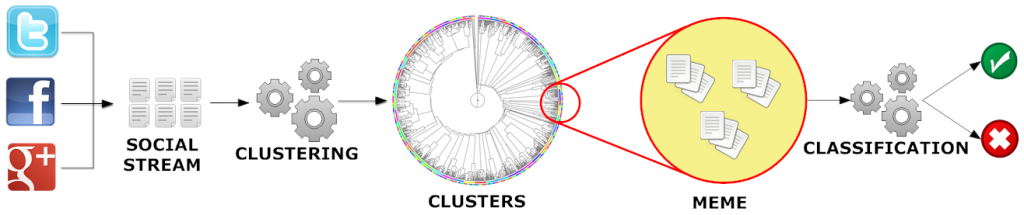
\includegraphics[width=5.8894in,height=1.2114in]{figures/chap3/chapitre3-img6.png}
    \caption{Algorithme de reconnaissance de mème (clustering) \citep{Ferrara2013}}
\end{figure}

Cet algorithme suppose donc d{\textquoteright}extraire dans un premier temps les éléments remarquables du corpus de tweets afin d{\textquoteright}établir des représentations de ces protomèmes contenant les éléments à comparer : \textit{phrases} (texte brut), \textit{mentions }(@, RT), \textit{hashtags }et \textit{urls}. Pour constituer ces jeux de protomèmes, nous utilisons le pattern \textit{map-reduce} qui permet de chercher et lister des éléments dans un vaste jeu de données \textit{(map)} avant de les regrouper dans une liste \textit{(reduce)}. Une fois ces protomèmes constitués nous procédons à leurs comparaisons selon plusieurs critères :

\begin{itemize}
\item \textit{Similarité de texte }: comparant le contenu texuel de chaque protomème 
\item \textit{Similarité d{\textquoteright}utilisateurs} : comparant les utilisateurs contenus dans chaque protomème
\item \textit{Similarités de tweet }: recherchant les tweets identiques dans différents protomèmes
\item \textit{Similarité de diffusion : }considérant les références aux utilisateurs contenus dans chaque protomème
\end{itemize}

Ici nous utilisons la \textit{sémantique vectorielle} (Support Vector Machine) afin de comparer les éléments des protomèmes gr\^ace à une représentation algébrique sous formes de vecteurs. Pratique ancienne de l{\textquoteright}algèbre linéaire appliquée à la science informatique \citep{Salton1975}, il s{\textquoteright}agit de permettre la conversion d{\textquoteright}objets textuels (mots, identifiants, images...) sous une forme aisément comparable. Pour convertir le texte sous forme vectorielle, l{\textquoteright}algorithme classique Tf-idf (\textit{Term Frequency - Inverse Document Frequency}) est utilisé \citep{Soucy2005}. Les autres mesures de similarité sont la \textit{mesure cosine (}ou \textit{similarité cosinus) }des protomèmes convertis sous forme de vecteurs binaires. Une fois ces différentes valeurs de similarité calculées, nous utilisons les scalaires définis dans le papier de référence pour assigner des poids à chacun des vecteurs et les combiner en une seule valeur \citep{Ferrara2013}. Cette matrice de valeurs de similarité nous permet alors de définir les protomèmes les plus similaires et d{\textquoteright}identifier ainsi des \textit{clusters }dans les données correspondant aux mèmes.


Si cette approche offre des résultats probants sur de petits volumes (quelques centaines de tweets), la très grande demande en puissance de calcul et ressources mémoires nécessaires rendent le traitement d{\textquoteright}un jeu données plus vaste irréalisable. Les opérations de comparaison et le calcul de similarités sur de vastes volumes de données font cro\^itre très rapidement la complexité des algorithmes et ainsi la quantité de calculs à effectuer. Le calcul du co\^ut d{\textquoteright}un algorithme se fait au travers des notions dites de domination, avec notamment le {\textquotedblleft}grand O{\textquotedblright} exprimé \textit{O(f(n)) }qui fait correspondre à la complexité d{\textquoteright}un algorithme une fonction \textit{f} de la quantité d{\textquoteright}information manipulée \textit{n. }Ainsi pour un algorithme courant de complexité \textit{O(n}\textit{\textsuperscript{2}}\textit{), }les ressources de calcul \textit{(computation)} et de mémoire (RAM ou stockage) nécessaires augmentent de manière exponentielle à chaque élément ajouté au corpus \textit{n}. L{\textquoteright}algorithme de {\textquotedblleft}meme clustering{\textquotedblright} décrit par Ferrara atteint donc un co\^ut exorbitant devant un large volume de données comme celui du jeu Weibosope. La limite physique de calcul est rapidement atteinte rendant impossible le franchissement du pallier expérimental et la vérification des hypothèses de travail à une échelle suffisante.

\subsection[ L{\textquoteright}identification des mèmes par hashtags ]{L{\textquoteright}identification des mèmes par hashtags }

Les travaux en sciences humaines sur les mèmes \citep{Bauckhage2011, Coscia2013, Knobel2007} et les sites spécialisés \citep{Buchel2012, Bernstein2011} présentent bien souvent un mème sous la forme d{\textquoteright}un titre (mot ou groupe de mots) accompagné d{\textquoteright}une collection d{\textquoteright}images ou/et de vidéos, ainsi qu{\textquoteright}un texte explicatif (mise en contexte) et des indications sur les dates de parution et son évolution dans le temps. Ici, un ou des auteurs se saisissent des matériaux bruts du web et les rassemblent pour reconstituer une vision particulière du mème, aussi représentative que possible. Cette approche nécessite peu de déploiement technologique (un copier/coller suffit souvent), mais exige néanmoins une forte connaissance et un suivi régulier du terrain Internet pour y dénicher ces représentations du mèmes. Cette démarche que nous nommerons \textit{ethnographique }s{\textquoteright}apparente à de la curation de contenu \citep{Buckingham2006}. Les \textit{hashtags }(en fran\c{c}ais {\textquotedblleft}mots-dièses{\textquotedblright}) sont utilisés dans l{\textquoteright}écriture sur les réseaux sociaux et se présentent dans Sina Weibo sous la forme d{\textquoteright}un mot entouré de deux dièses - ex. \textit{\#mot-clé\#}. Marqueur particulier, le hashtag permet à un interlocuteur de procéder à une dénotation ou connotation du message original \citep{Romero2011} ou d{\textquoteright}affirmer son caractère évènementiel (lors d{\textquoteright}un évènement sportif, d{\textquoteright}une conférence, etc). Facile à identifier dans la masse des données en ligne, il permet de désigner un ensemble de contenus sous un m\^eme signe. Ainsi, il est un vecteur important permettant de collecter simplement une large masse d{\textquoteright}informations autour d{\textquoteright}un mème. La constitution d{\textquoteright}un corpus autour d{\textquoteright}un {\textquotedblleft}hashtag{\textquotedblright} présente néanmoins plusieurs limites. Premièrement, le mème est par définition un objet en mutation. Ainsi, il est souvent difficile de l{\textquoteright}identifier une bonne fois pour toute par un ou plusieurs de mot-clés. De plus, le mème existe bien souvent sous la forme d{\textquoteright}images ou de vidéos qui ne sont pas nécessairement légendées ou référencées et donc peu accessible à une recherche {\textquotedblleft}plein texte{\textquotedblright}. Ainsi, une approche pour la recherche de mèmes ne peut \^etre entièrement textuelle et doit s{\textquoteright}intéresser aux autres forme de contenus web (notamment les liens et les hashtags). De plus, l{\textquoteright}ajout de hashtags dans les messages est un acte volontaire non systématique. Ainsi, si l{\textquoteright}identification de certains mèmes peut se faire gr\^ace à la recherche de hashtags, l{\textquoteright}ensemble des messages contenant des hashtags ne recouvrent pas systématiquement un mème. Comme nous le verrons, les hashtags sont bien souvent de simples artefacts de campagne marketing en ligne.

Afin de procéder à l{\textquoteright}analyse des mèmes, nous avons donc indexé l{\textquoteright}ensemble des contenus du corpus Weiboscope contenant des hashtags sur toute l{\textquoteright}année 2012 (30 millions sur un total de 200 millions tweets environs). Nous avons donc dans un premier temps extrait l{\textquoteright}ensemble des messages contenant un ou des hashtags de l{\textquoteright}ensemble des données avant de les classifier pour obtenir des jeux de données cohérents par hashtags. Une première contrainte ici est propre au traitement informatique de la langue chinoise qui constitue le langage majoritaire de notre corpus. L{\textquoteright}absence d{\textquoteright}espace entre les différents caractères de la phrase en chinois oblige à prendre en compte la sémantique de la phrase pour procéder à sa segmentation. Cette question usuelle pour les usagers du NLP (\textit{Natural Language Processing}) en chinois est un sujet de recherche encore très discuté \citep{Qiu2013}. L{\textquoteright}identification de la meilleure option parmi la multitude des librairies et logiciels disponibles pour la segmentation puis le NLP en chinois a été un aspect préliminaire importants de notre travail d{\textquoteright}analyse de données. Nous avons ainsi réalisé de nombreux benchmark afin de comparer les différentes technologies existantes. Un travail mené avec l{\textquoteright}équipe du site Internet d{\textquoteright}actualité scientifique \textit{Guokr }à Pékin nous a amené à choisir en premier lieu un algorithme de segmentation développé sur la base de textes en chinois ancien\footnote{ gkSeg : \textit{{\textquotedblleft}Yet another Chinese word segmentation package based on character-based tagging heuristics and CRF algorithm{\textquotedblright} }\url{https://github.com/guokr/gkseg}, consulté le 14 Mars à 18:28}. Après plusieurs tentatives, nous avons préféré le segmenteur open-source Jieba\footnote{ \url{https://github.com/fxsjy/jieba}, consulté le 14 Mars à 18:30} plus généreux en termes de fonctionnalités et permettant de meilleures performances. Une fois la phrase chinoise segmentée, la seconde étape consiste à supprimer tous les mots les plus communs \textit{(stopwords)}, ainsi que la ponctuation et d{\textquoteright}autres caractères trop courants afin de préserver uniquement les mots riches de sens dans les phrases (les mots-clés). L{\textquoteright}extraction des hashtags est effectuée gr\^ace à une expression régulière qui scanne le texte pour identifier et préserver uniquement les caractères situés entre les deux signes dièse (\#). Sur un total d{\textquoteright}environ 30 millions de tweets contenant des hashtags, nous avons choisi de retenir seulement les hashtags possédant plus de 1000 messages. Nous avons ensuite décidé d{\textquoteright}ignorer les 1000 hashtags les plus utilisés car ils ne présentaient pas d{\textquoteright}intér\^et pour notre étude, étant la plupart du temps des noms de marque ou des mots-clés trop généraux (par exemple : {\textquotedblleft}bonne nuit{\textquotedblright}, {\textquotedblleft}nouvelles de sports{\textquotedblright}, {\textquotedblleft}photos de nourriture{\textquotedblright}, etc).

\begin{figure}[ht]
    % \centering
    
    \begin{minipage}[b]{0.5\linewidth}
        \centering
        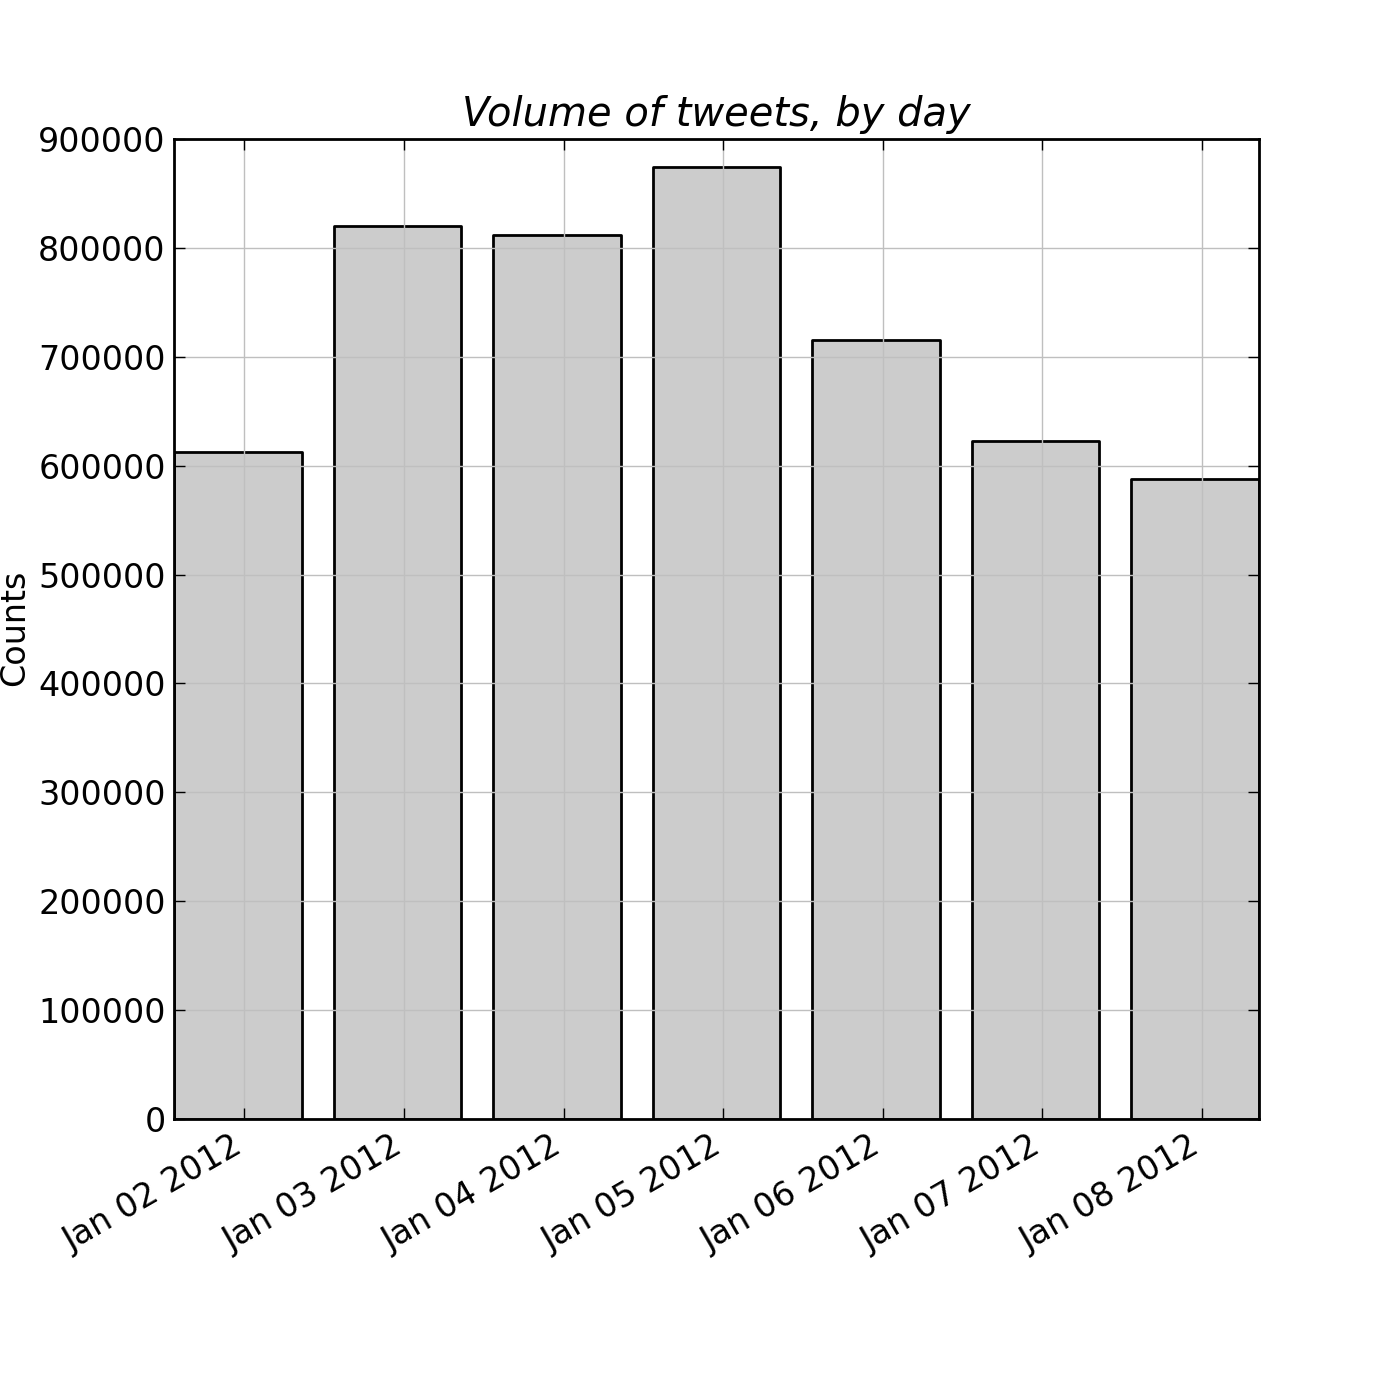
\includegraphics[width=3.2004in,height=3.2004in]{figures/chap3/chapitre3-img7.png}
        \caption*{Volume de tweets}
        \par\vspace{0pt}
    \end{minipage}%

    \hspace{0.5cm}

    \begin{minipage}[b]{0.45\linewidth}
        \centering
        \begin{tabular}{c|c|c|c}
            \textit{hashtags} & \textit{users} &  \textit{actions} & \textit{tweets} \\
            \hline\\ [-1ex]
            \zh{吴奇隆} & 201 & 13243 & 22349  \\
            \zh{一起到老} & 182 & 0 & 364  \\
            \zh{春运} & 92 & 13 & 256  \\
            \zh{轻松一刻} & 92 & 11 & 240  \\
            \zh{人品值分析} & 90 & 490 & 321  \\
            \zh{朝阳区} & 88 & 49 & 165  \\
            \zh{理性态小度} & 87 & 0 & 329  \\
            \zh{美图GIF} & 87 & 101 & 404  \\
            \zh{我正在听} & 86 & 6 & 330  \\
            \zh{微盘签到} & 84 & 304 & 305  \\
            \zh{2012来了} & 83 & 206 & 309  \\
            \zh{中级达人} & 83 & 0 & 159  \\
            \zh{分享} & 82 & 87 & 563  \\
            \zh{星座} & 82 & 5 & 195  \\
        \end{tabular}
        \caption*{Hashtags les plus utilisés}
        \par\vspace{0pt}
    \end{minipage}%
        
    \caption[Volume de tweets et hashtags pendant la 1ère semaine de 2012]{\textit{Volume de tweets et hashtags pendant la 1ère semaine de 2012} - Les résultats concernant la 1ère semaine de l{\textquoteright}année 2012 donnent un aper\c{c}u du volume analysé : 5,044,331 tweets, 398 392 utilisateurs uniques cités (dans un total de 2 115 544 mentions), 264 651 urls uniques (pour un total de 426 914) et 44 382 hashtags uniques (pour un total de 244285).}

\end{figure}


Notre étude vise à analyser les dynamiques conversationnelles et nous devons donc déterminer les plus adéquats parmi des hashtags de nature souvent très différentes. Pour ce faire, nous avons sélectionné pour chaque jeu de données (chaque hashtag) deux mesures significatives : premièrement, le volume de messages ; deuxièmement, la quantité d{\textquoteright}échanges et d{\textquoteright}interactions effectives entre les utilisateurs (commentaires, retweets, etc.). Ces deux mesures nous permettent de nous assurer que 1) nous possédons une quantité suffisante de messages pour mener à bien l{\textquoteright}étude et que 2) la discussion a bien eu lieu et qu{\textquoteright}il ne s{\textquoteright}agit pas de messages redondants ou non reliés entre eux. Nous avons choisi d{\textquoteright}ignorer les échanges dominés à plus de 80\% par le m\^eme utilisateur pour éviter la pollution de l{\textquoteright}étude par l{\textquoteright}activité de robots. Le graphe ci-dessous permet d{\textquoteright}observer la distribution de 429 hashtags possédant tous plus de 1000 tweets et 1000 échanges : l{\textquoteright}axe vertical représente la quantité d{\textquoteright}actions (échanges) et l{\textquoteright}axe horizontal le volume des conversations. Tout en bas du graphe se trouvent donc les hashtags ayant été les moins discutés, avec en haut ceux aux conversations les plus intenses. La taille des points illustre le volume de messages et la couleur la quantité de conversations.
% je ne comprends pas le code couleur % 

\begin{figure}
    \centering
    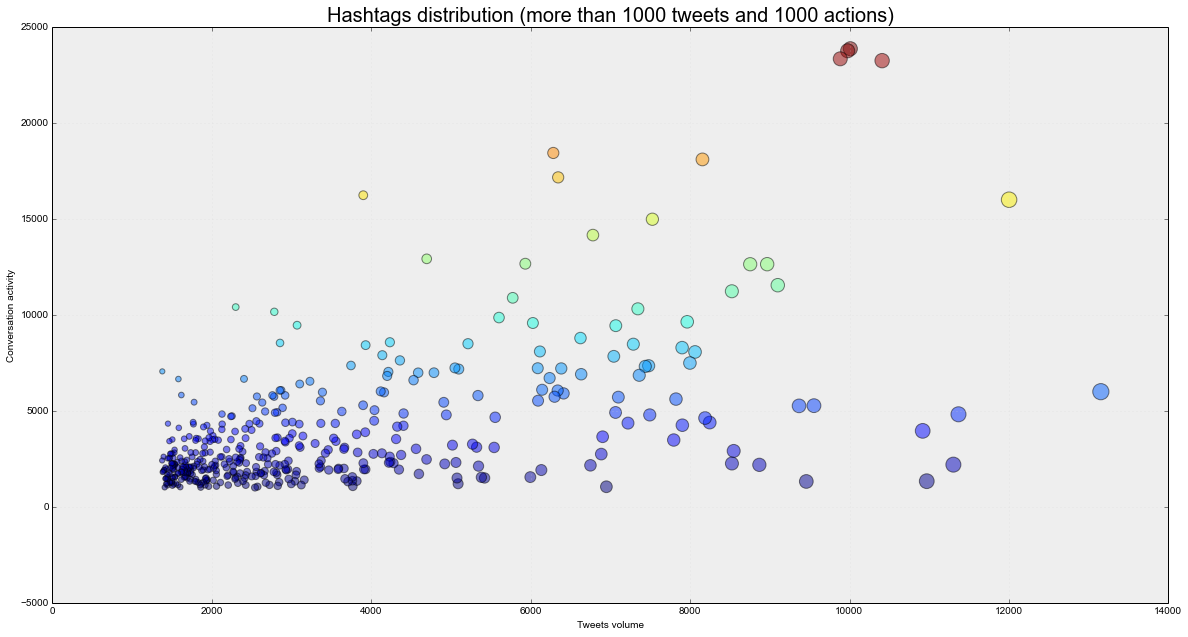
\includegraphics[width=6.0114in,height=3.2114in]{figures/chap3/chapitre3-img8.png}
    \caption{Distribution des 429 hashtags les plus discutés}
\end{figure}


En procédant à l{\textquoteright}étiquetage des hashtags les plus actifs durant l{\textquoteright}année 2012 sur Sina Weibo (figure 2 ci-dessus), nous constatons que la plupart sont associés à des activités commerciales, de loisirs ou de divertissement. Ici nous observons que les usages majoritaires du réseau social Sina Weibo correspondent pour la plupart à ceux d{\textquoteright}autres mass-médias plus traditionnels de par le monde. Le commerce en ligne occupe notamment une place proéminente. La marque de téléphonie mobile chinoise \textit{Xiaomi }est abondamment citée, reflétant son importance croissante dans le marché chinois et surtout sa stratégie commerciale qui cible abondamment les réseaux sociaux avec de nombreux hashtags très discutés (notamment \textit{{\textquotedblleft}Fans de Xiaomi{\textquotedblright} }[5C0F?][7C73?][7C89?][4E1D?] ). Également, de nombreuses campagnes promotionnelles d{\textquoteright}ouverture ou d{\textquoteright}anniversaire de magasins ont réussi à se hisser dans le jeu de t\^ete des hashtags les plus discutés. Radio-crochets ou chanteurs reconnus, les stars de la télévision et de la chanson sont aussi présents dans le peloton de t\^etes des discussions sur Sina Weibo. Le célèbre chanteur Han Geng notamment compte près d{\textquoteright}une dizaine de hashtags le concernant parmi les 500 les plus discutés (\textit{{\textquotedblleft}Han Geng fait une pub pour Nokia{\textquotedblright}, {\textquotedblleft}Han Geng va en Italie{\textquotedblright}, {\textquotedblleft}Han Geng fait une pub Pepsi{\textquotedblright}, {\textquotedblleft}Han Geng refuse une interview{\textquotedblright}, etc.)} Ici encore, le réseau social agit comme le prolongement des mass média traditionnels, élément-clé des nouvelles stratégies de publicités en ligne, parfois particulièrement agressives comme dans le cas de Han Geng. Les contenus de la télévision sont largement relayés et discutés, notamment les séries télévisuelles. Le cinéma est aussi représenté. Le film comique chinois \textit{Lost in Thailand }sorti en Décembre 2012 dépeint les aventures d{\textquoteright}un chinois en vacances en Thailande. Premier grand succès commercial du box-office chinois, sa popularité se reflète dans l{\textquoteright}importance au sein des discussions en ligne. Les tendances des ventes du livre sont reflétées par de nombreux best-seller sur {\textquotedblleft}l{\textquoteright}amélioration de soi{\textquotedblright} ou la {\textquotedblleft}réussite économique{\textquotedblright}\textit{. }Ce type de hashtags ne se limite pas au support web mais s{\textquoteright}origine directement dans d{\textquoteright}autres médias plus traditionnels. Le gouvernement lui-m\^eme utilise Sina Weibo pour faire passer ses messages avec un hashtag \textit{{\textquotedblleft}information officielle{\textquotedblright} }utilisé notamment pour des démentis publics ou droit de réponse par l{\textquoteright}entreprise Sina, propriétaire du service. également outil de conversation, les discussions sur les réseaux sociaux parlent de la vie de tous les jours. La situation routière et les bouchons dans chaque ville sont un des grands sujets de discussions. Ce sont dans ces échanges quotidiens que se cristallisent plus particulièrement les enjeux politiques et médiatiques des réseaux sociaux. Nouveau café du commerce, les commentaires sur les faits divers et l{\textquoteright}actualité mettent souvent à jour les dysfonctionnements de systèmes politiques, urbains ou légaux. Il est intéressant néanmoins de noter que parmi les hashtags les plus discutés, les phénomènes de suppression de contenus par les administrateurs (censure) restent très marginal. Le \textit{China Digital Times} de UC Berkeley maintient une liste des mots interdits sur Sina Weibo depuis plusieurs anneés \citep{Ng2013}. En comparant cette liste de mots censurés à celle des hashtags, nous avons pu voir qu{\textquoteright}aucun des 3000 hashtags les plus utilisés en 2012 n{\textquoteright}a été soumis a une interdiction m\^eme temporaire sur Sina Weibo. Les hashtags les plus sujets à la censure ne sont pas en lien avec des domaines politiques ou des sujets sensibles, mais plut\^ot avec des contenus à caractère pornographique (la pornographie est interdite en Chine). Reflétant les usages majoritaires (commerce, loisirs, etc.), les hashtags véhiculent des contenus souvent moins controversés et les {\textquotedblleft}mots censurés{\textquotedblright} sont plus à m\^eme d{\textquoteright}appara\^itre dans des discussions informelles.

\subsection[Visualisation du graphe conversationnel d{\textquoteright}utilisateurs]{Visualisation du graphe conversationnel d{\textquoteright}utilisateurs}

Après avoir identifié différents \textit{mèmes parmi }les hashtags les plus discutés de l{\textquoteright}année 2012, nous allons maintenant procéder à l{\textquoteright}analyse du déroulement des échanges d{\textquoteright}après chacun des différents corpus de données. Plusieurs types de graphes peuvent \^etre extraits :

\begin{itemize}
\item \textbf{Graphe social statique}: représentant les relations pré-existantes dans la structure du réseau étudié (untel est ami avec untel, untel suit untel, etc.)
\item \textbf{Graphe conversationnel}: représentant toutes les interactions qui entourent et structurent la diffusion de messages 
\item \textbf{Graphe de diffusion}: représentant les interactions qui se sont produites entre les acteurs durant \ la diffusion du message. Ce dernier type de graphe est un recoupement des deux autres.
\end{itemize}


\begin{figure}
    \centering
    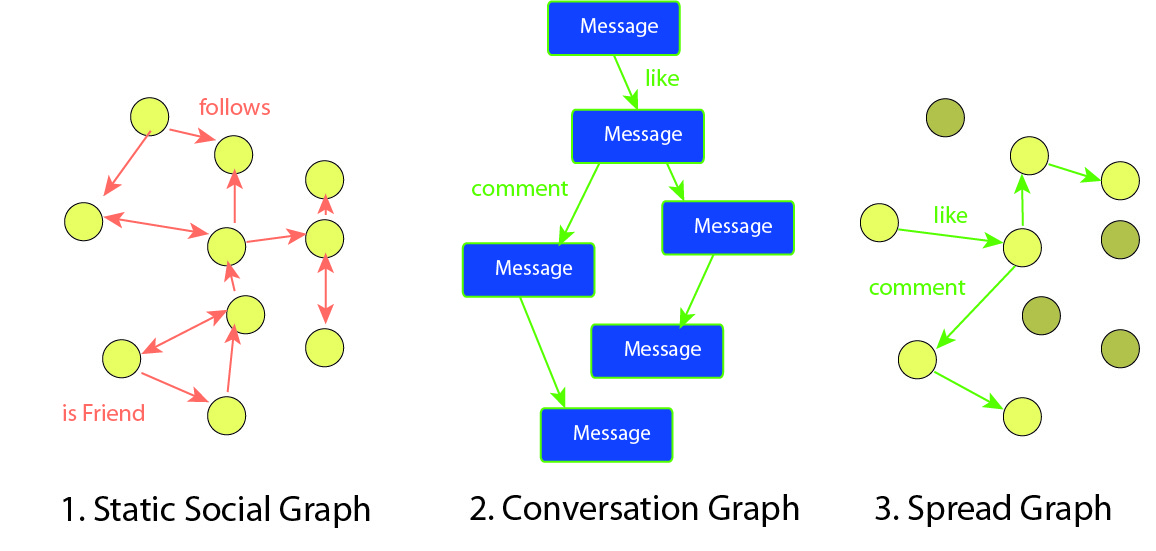
\includegraphics[width=6.2894in,height=3.0004in]{figures/chap3/chapitre3-img9.jpg}
    \caption[3 modèles de réseau]{Les 3 types de graphe classiquement extraits des données de réseaux sociaux}
\end{figure}


Dans notre étude, le graphe social statique ne présente pas particulièrement d{\textquoteright}intér\^et puisqu{\textquoteright}il correspond à un ensemble de relations peu affecté par les discussions. De plus, nous ne disposons dans le jeu de données Weiboscope que de son état final qui ne témoigne pas de l{\textquoteright}évolution des relations. Nous voulons obtenir ici les graphes de diffusion sous la forme de conversations structurées\textbf{~(}graphe directionnelle des \ réponses et commentaires) de l{\textquoteright}ensemble des messages. Dans un article paru dans \textit{Nature} \citep{Weng2012}, les chercheurs du \textit{Centre de Recherche sur les Systèmes Complexes} de l{\textquoteright}Université d{\textquoteright}Indiana identifient les caractéristiques des mèmes connaissant le plus de succès (la plus large diffusion). Un travail de visualisation de mèmes identifiés par des hashtags sur Twitter leur permet notamment de mettre à jour des motifs particuliers dans la structure des conversations.


\begin{figure}[ht]
    \centering
    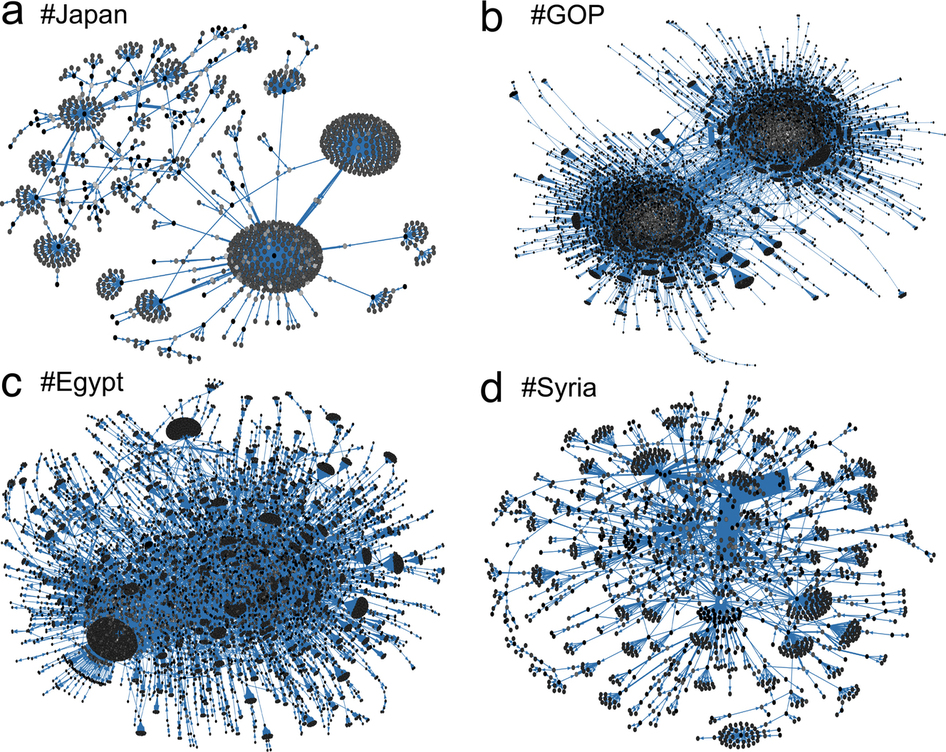
\includegraphics[width=5.5669in,height=4.4224in]{figures/chap3/chapitre3-img10.jpg}

    Nodes represent Twitter users, and directed edges represent retweeted posts that carry the meme. The brightness of a node indicates the activity (number of retweets) of a user, and the weight of an edge reflects the number of retweets between two users. \newline
    (a) The \textit{\#Japan}  meme shows how news about the March 2011 earthquake propagated. \newline
    (b) The \textit{\#GOP} tag stands for the US Republican Party and as many political memes, displays a strong polarization between people with opposing views. \newline
    Memes related to the Arab Spring and in particular the 2011 uprisings in (c) \textit{\#Egypt} and (d) \textit{\#Syria} display characteristic hub users and strong connections, respectively.
    
    \caption{Graphe de diffusion de hashtags sur Twitter d{\textquoteright}après \citep{Weng2012} }

\end{figure}


Afin de mettre à jour le graphe conversationnel entourant les hashtags
sélectionnés sur Sina Weibo, nous avons choisi
d{\textquoteright}extraire la séquence d{\textquoteright}interactions
des messages (mentions, retweets) composant chaque mème. Cette
structure de graphe nous permet de représenter la diffusion de chaque
mème sous forme d{\textquoteright}un graphe contenant un node par
utilisateur et un ensemble de relations correspondant aux échanges
visibles dans les textes des messages. Dans un premier temps, le
logiciel \textit{Graphviz }nous a permis d{\textquoteright}obtenir une
représentation basique du graphe conversationnel afin
d{\textquoteright}avoir un aper\c{c}u sur la nature des conversations
par l{\textquoteright}observation des motifs qui la compose. En effet,
si les deux mesures identifiées à l{\textquoteright}étape
précédente (volume de messages et \ volume
d{\textquoteright}échanges) nous permettent
d{\textquoteright}effectuer un premier tri parmi les hashtags, cette
première visualisation nous permet de considérer la nature des
échanges et l{\textquoteright}implication des utilisateurs
d{\textquoteright}après la structure des motifs conversationnels.
Chaque utilisateur est symbolisé par un point et chaque message par
un trait reliant deux utilisateurs. Un motif très compact reflète
une conversation animée entre des utilisateurs peu nombreux
échangeant beaucoup. A l{\textquoteright}inverse, un motif disparate
reflète des échanges plus brefs et morcelés.

\begin{figure}[ht]
    
    \begin{minipage}[b]{0.4\linewidth}
        \centering
        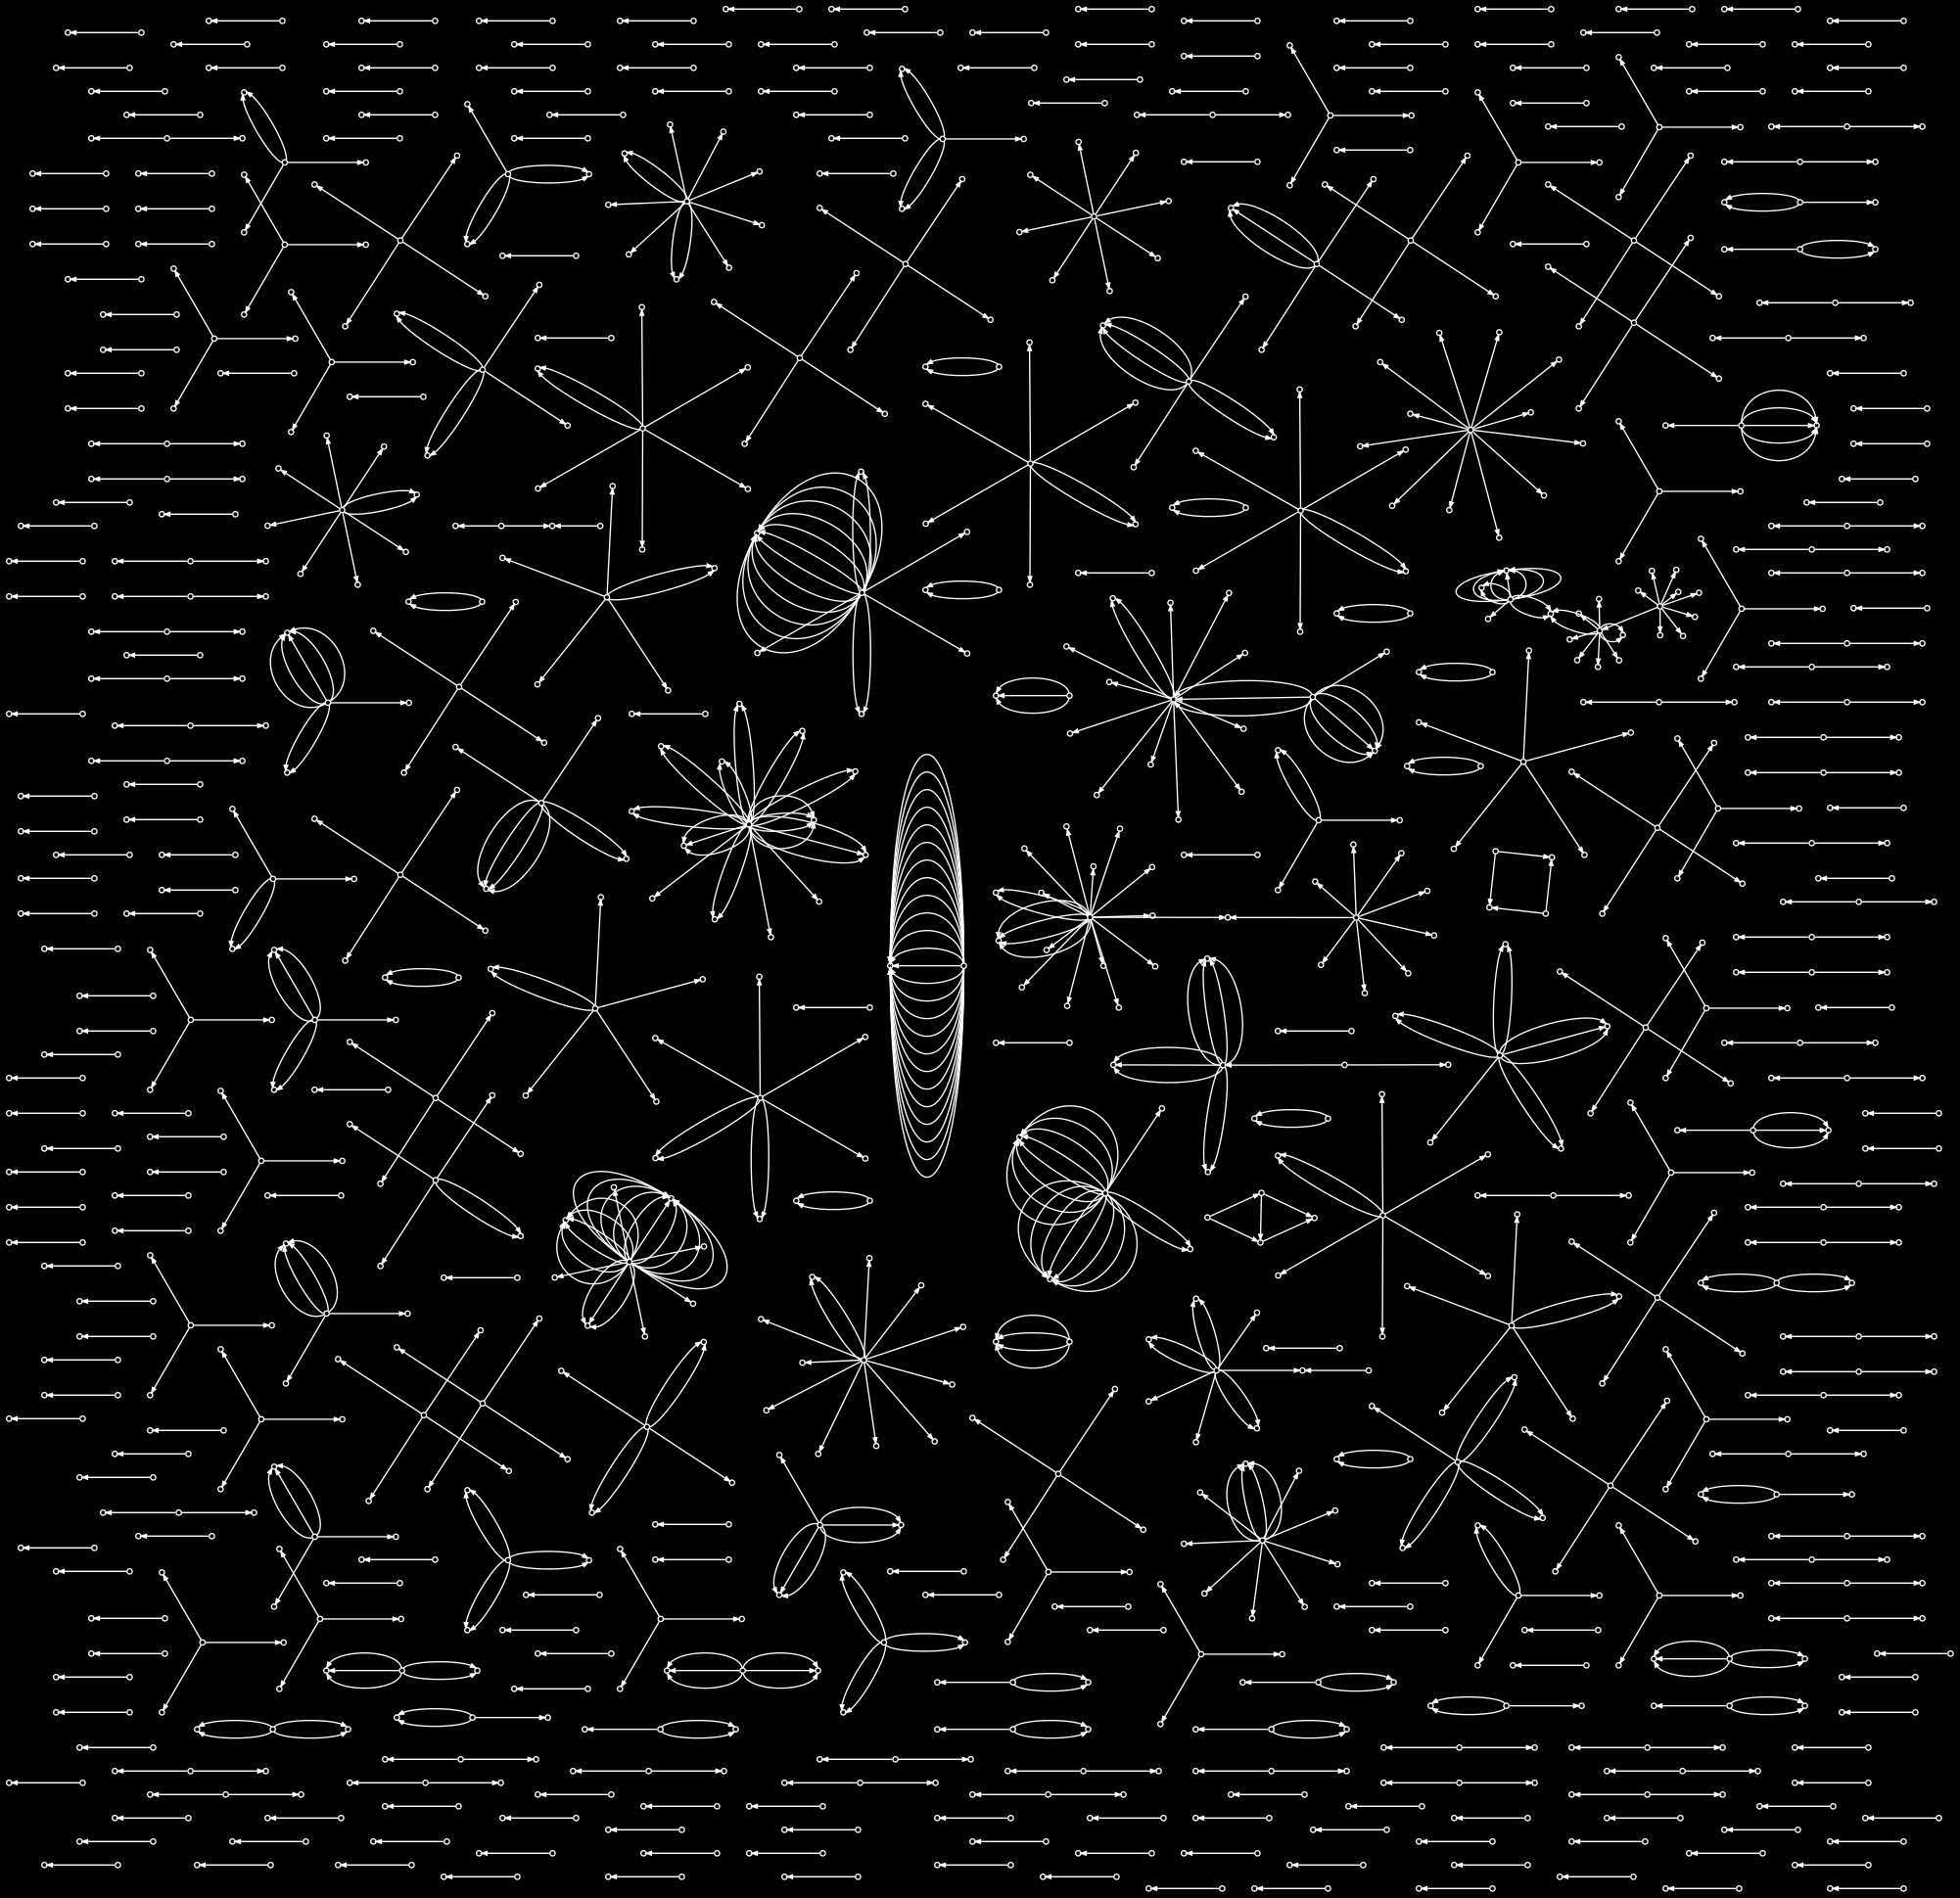
\includegraphics[width=2.5in,height=2.5in]{figures/chap3/chapitre3-img11.png}
        \par\vspace{0pt}
    \end{minipage}
    \begin{minipage}[b]{0.55\linewidth}
        \centering
        \raggedright
        \textit{WeicoPlus }est une application mobile permettant
        d{\textquoteright}utiliser Sina Weibo. Le hashtag \#WeicoPlus\# est
        ajouté automatiquement quand les utilisateurs postent des photos
        depuis ce service. 

        Ainsi, on remarque que le graphe conversationnel
        entourant WeicoPlus se compose essentiellement de messages simples,
        mais ne donne pas lieu à une conversation structurée - à
        l{\textquoteright}exception de quelques rapides échanges entre un
        nombre réduit de personnes.
        \par\vspace{0pt}
    \end{minipage}

    \caption[Visualisation simple du hashtag{\textquotedblleft}WeicoPlus{\textquotedblright}] {Fig. Visualisation simple du hashtag{\textquotedblleft}WeicoPlus{\textquotedblright}, un trait représente un échange entre deux utilisateurs}
\end{figure}




\begin{figure}[ht]
    \begin{minipage}[b]{0.4\linewidth}
        \centering
        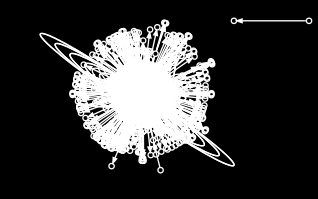
\includegraphics[width=2.5in,height=1.5in]{figures/chap3/chapitre3-img12.png}
        \par\vspace{0pt}
    \end{minipage}
    \begin{minipage}[b]{0.55\linewidth}
        \centering
        \raggedright
        A l{\textquoteright}inverse, le hashtag {\textquotedblleft}Veuve
        d{\textquoteright}enfant
        unique{\textquotedblright} \zh{\#失独母亲\#} cristallise
        le débat en une forme très dense qui reflète une surenchère de
        commentaires et d{\textquoteright}actions autour du hashtag, propre
        d{\textquoteright}une conversation animée. 
        \par\vspace{0pt}
    \end{minipage}

    \caption[Visualisation simple des conversations autour du hashtag Veuve d{\textquoteright}enfant unique]{Visualisation simple des conversations autour du hashtag Veuve d{\textquoteright}enfant unique}
\end{figure}


\subsection[Premiers éléments d{\textquoteright}analyse: visualisation de mèmes ]{Premiers éléments d{\textquoteright}analyse: visualisation de mèmes }

Les différents modèles de conversation que nous obtenons dans cette première étape se présentent sous une forme schématique et peu détaillée. Afin de comprendre plus en détails les dynamiques conversationnelles qui les entourent, nous avons choisi de sélectionner trois exemples parlants de hashtags dont les graphes conversationnels présentent des particularités des modèles de diffusion dissemblables et organisés. Pour chacun d{\textquoteright}eux, nous allons procéder à une analyse plus détaillée des graphes conversationnels afin de considérer les différences entre ces différents modèles.


\begin{figure}[th]
    \centering
    \subfloat[Pluie torrentielle à Tianjing]{
        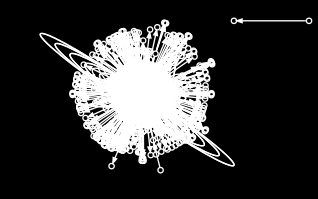
\includegraphics[width=2.3224in,height=1.4449in]{figures/chap3/chapitre3-img13.png}
    }

    \subfloat[Veuve à l{\textquoteright}enfant unique]{
        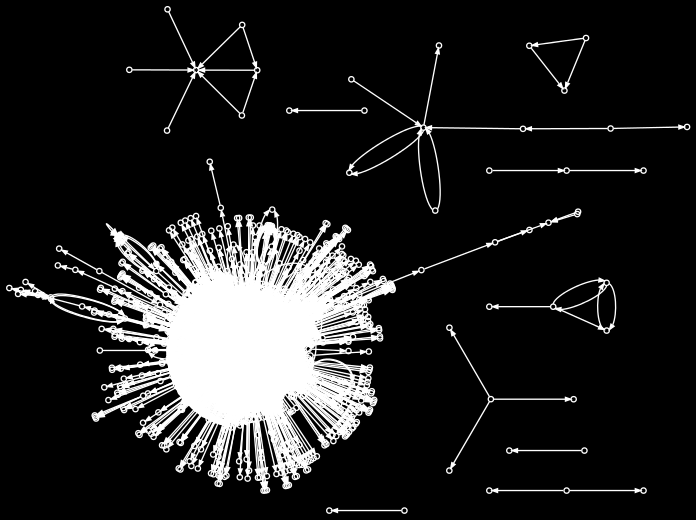
\includegraphics[width=2.3004in,height=1.7224in]{figures/chap3/chapitre3-img14.png}
    }

    \subfloat[Abolition des lois sur la prostitution]{
        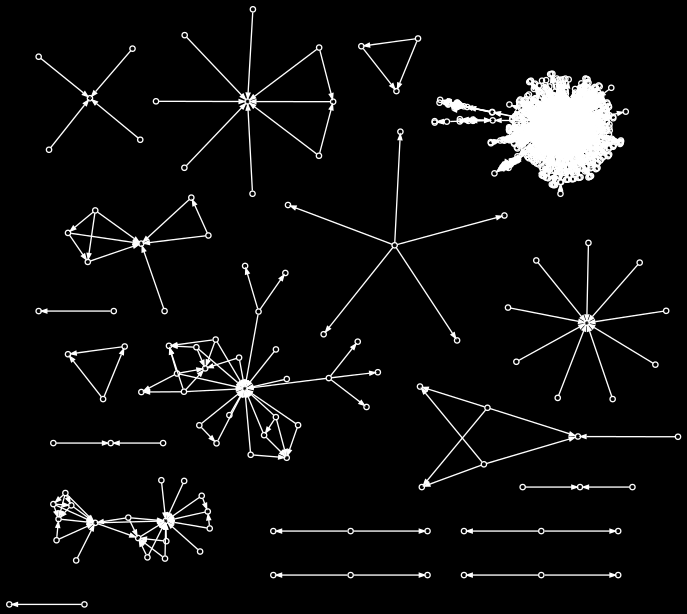
\includegraphics[width=2.1449in,height=1.9224in]{figures/chap3/chapitre3-img15.png}   
    }
  
    \caption{Visualisation des conversations autour de trois hashtags}
\end{figure}


Nous voyons que les trois représentations des graphes ci-dessus donnent à voir des structures plus ou moins morcelées, avec un ensemble de points et de lignes très compactes qui représentent la majeure partie de la conversation. Afin de visualiser plus précisément les groupes et les dynamiques qui constituent les discussions autour de chaque hashtag, nous allons utiliser le logiciel Gephi \citep{Bastian2009} afin d{\textquoteright}examiner de plus près la composition de ces graphes. Pour ce faire, Gephi va nous permettre d{\textquoteright} {\textquotedblleft}étaler{\textquotedblright} le graphe en repositionnant les nodes et en les coloriant pour en identifier les composantes et les tendances.

Chaque utilisateur est représenté sous la forme d{\textquoteright}un point. La taille des points correspond à l{\textquoteright}importance de l{\textquoteright}utilisateur dans le réseau total des échanges, caractérisé par son degré de centralité intermédiaire (\textit{betweenness centrality}), une mesure topologique correspondant au nombre de plus courts chemins du graphe passant par cet utilisateur. La couleur est utilisée pour représenter la \textit{modularité }du réseau, c{\textquoteright}est à dire le nombre de communautés engagées dans la conversation définies comme les cliques d{\textquoteright}utilisateurs constituant plus de 1\% du réseau total d{\textquoteright}échange \citep{Blondel2008}. La position des nodes est calculée gr\^ace à l{\textquoteright}algorithme \textit{Force Atlas 2} \citep{Bastian2009} utilisant une modélisation physique o\`u les nodes peu connectés entre eux se repoussent et ceux très connectés s{\textquoteright}attirent. Ainsi, la proximité de deux nodes sur le graphe témoigne d{\textquoteright}une proximité lors des conversations, c{\textquoteright}est à dire de l{\textquoteright}existence d{\textquoteright}un échange entre eux (citations, commentaires ou retweets). Pour davantage de visibilité, certaines conversations sub-alternes représentant moins de 1\% du total ont été effacées. Egalement, les nodes possédant un degré inférieur à 3 (moins d{\textquoteright}un échange avec au moins trois autres nodes du grahe) ne sont pas représentés.


\textbf{Exemple 1 : Pluie torrentielle à Tianjing}

Le premier mème choisi parle d{\textquoteright}une catastrophe naturelle, sous la forme d{\textquoteright}une pluie diluvienne qui s{\textquoteright}est abattue sur la ville de Tianjin durant la nuit du 21 au 22 Juillet 2012.

\begin{figure}
    \centering
    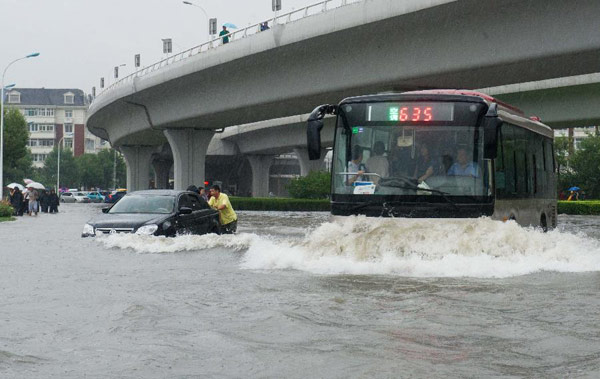
\includegraphics[width=6.0114in,height=3.7894in]{figures/chap3/chapitre3-img16.jpg}
    \caption[Photo de Tianjin durant la pluie torentielle en Juillet 2012]{\textit{Downpour bypasses Beijing, batters neighbor, }in Qinghua News le 2012-07-26 13:29:59, \url{http://news.xinhuanet.com/english/china/2012-07/26/c_131740415.htm} consulté le 27 Juin 2014.}
\end{figure}

Ici 4 groupes composent 85\% du graphe, constitués autour de gros diffuseurs (les nodes les plus gros). Plusieurs groupes semblent s{\textquoteright}emparer de la conversation mais on voit peu d{\textquoteright}activité entre les nodes alors que les échanges se déroulent autour de quelques utilisateurs très centraux. Cela traduit le fait que peu de personnes ont réellement discuté l{\textquoteright}information et elles se sont simplement contentées de la relayer.

\begin{figure}[th]
    \centering
    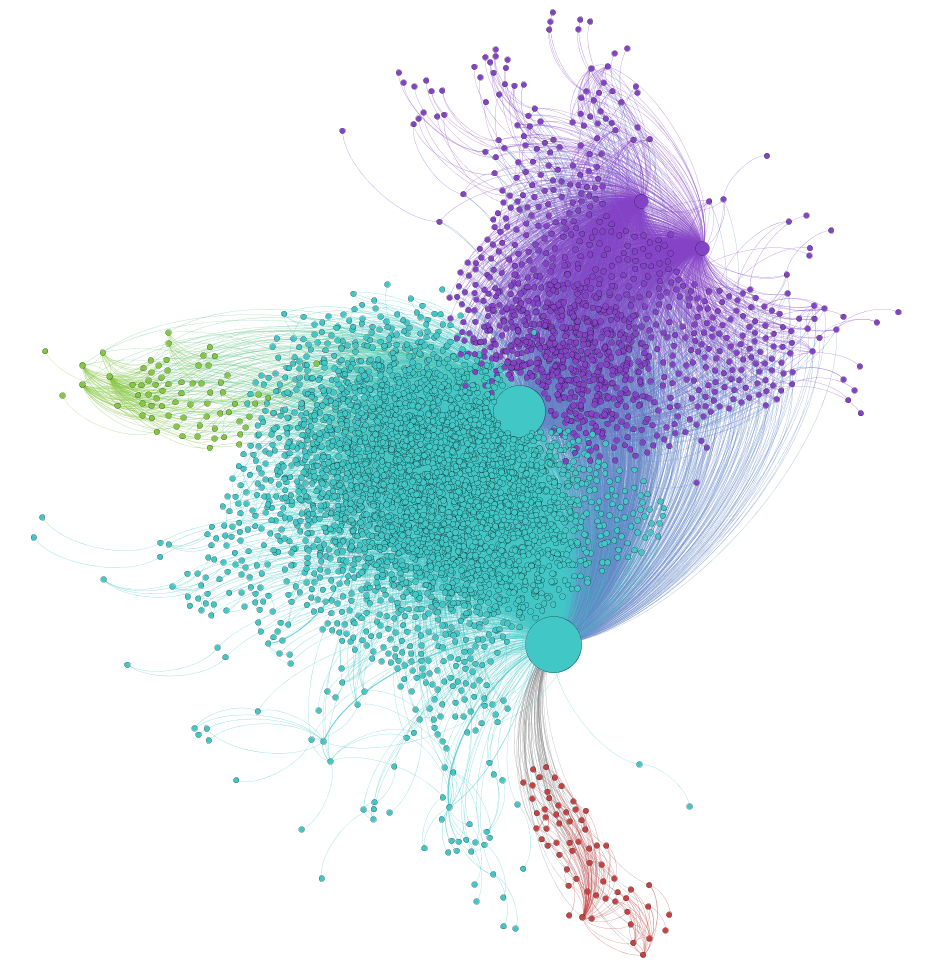
\includegraphics[width=6.0114in,height=6.0114in]{figures/chap3/chapitre3-img17.png}
    \caption{Exemple 1 : Tianjin Baoyu}
\end{figure}

La diffusion d{\textquoteright}un fait divers très local (il se passe à Tianjing) est entrainée par peu de sources très importantes (les quelques nodes de grande taille), vraisemblablement des journaux et médias locaux qui annoncent la nouvelle (presse, photos-choc d{\textquoteright}innondations, etc). La conversation est peu active et très structurée, nous sommes en présence d{\textquoteright}un modèle classique de diffusion de masse.

\textbf{Exemple 2 : Veuve de l{\textquoteright}enfant unique}

Un autre sujet discuté par une très large quantité de personnes appara\^it sous le terme {\textquotedbl}\textit{shidu muqin}{\textquotedbl}, forme contractée signifiant \textit{{\textquotedblleft}mère qui a perdu son enfant unique{\textquotedblright}} (\zh{\#失独母亲\#}). Ce hashtag désigne un phénomène de société bien connu en Chine o\`u le deuil de la perte d{\textquoteright}un enfant se double souvent pour une mère chinoise seule de l{\textquoteright}absence de ressources pour vivre. En effet, l{\textquoteright}absence de système de retraite fait porter aux enfants la responsabilité de la survie de la famille.

Le graphe ici est fait de deux grands groupes composant à eux deux
près de 95\% du graphe total. Les discussions sont très
polarisées et menées par peu de participants (les nodes les plus
gros sur le graphe). Peu de personnes très influentes concentrent les
discussions autour d{\textquoteright}eux, accompagnés ou suivis
d{\textquoteright}une foule de commentateurs. 

\begin{figure}[th]
    \centering
    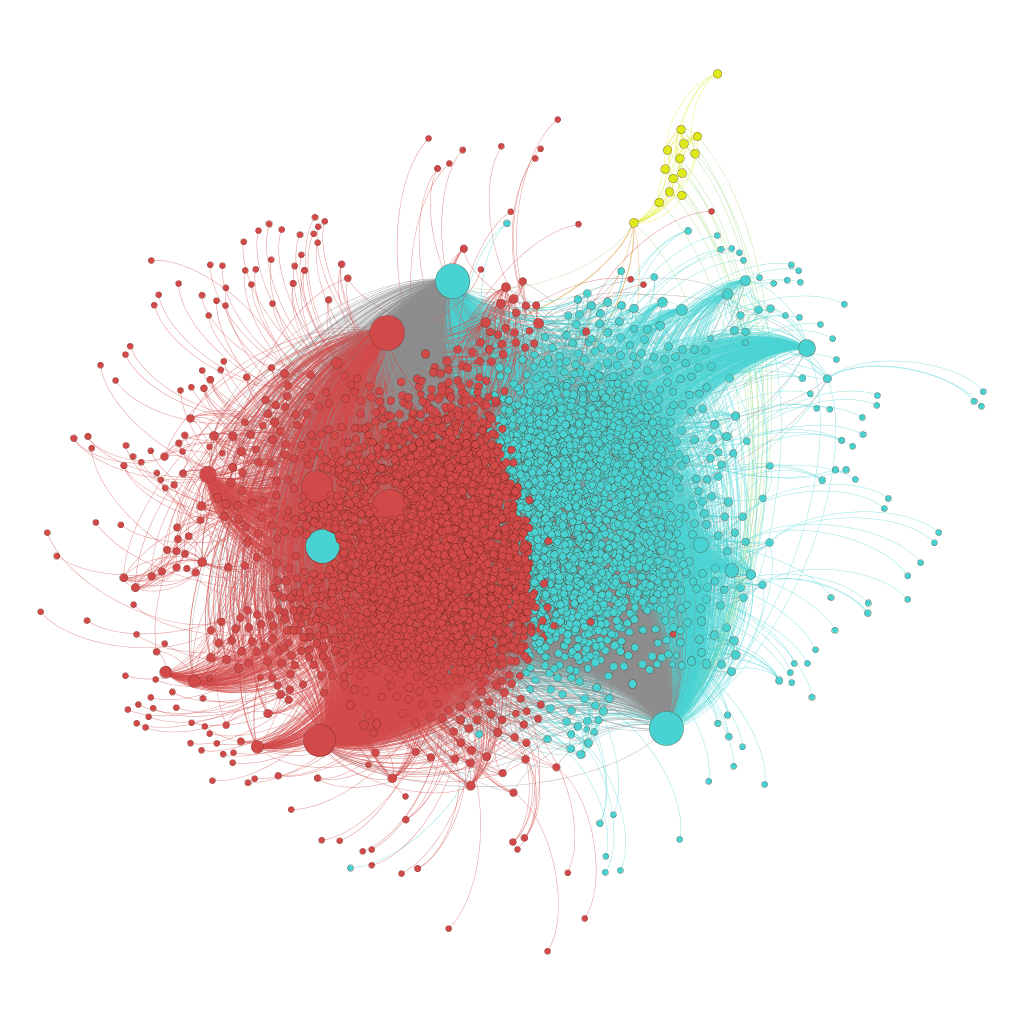
\includegraphics[width=6.0114in,height=6.0114in]{figures/chap3/chapitre3-img18.png}
    \caption{{\textquotedblleft}Shidu Muqin{\textquotedblright}}
\end{figure}


Cet exemple donne à voir des groupes bien définis et très proches o\`u plusieurs acteurs majeurs mènent la discussion. Les dynamiques d{\textquoteright}échanges autour d{\textquoteright}une question de société (la loi de l{\textquoteright}enfant unique en Chine et ses conséquences) s{\textquoteright}articule en groupes distincts sans pour autant amener à des controverses importantes (qui se traduiraient par des discussions longues et houleuses). Ici, les leaders d{\textquoteright}opinion font la discussion et la diffusion se fait au travers d{\textquoteright}eux.

\clearpage
\textbf{Exemple 3 : Abolition des lois sur la prostitution}

Le hashtag \textit{{\textquotedblleft}Abolissons la loi piaowudong nuzui{\textquotedblright} }est l{\textquoteright}expression d{\textquoteright}une campagne pour l{\textquoteright}abolition d{\textquoteright}une législation scandaleuse sur la prostitution en Chine. Depuis les années 80, la loi chinoise interdit la prostitution et prévoit la condamnation des deux parties qui s{\textquoteright}adonnent à un échange d{\textquoteright}argent. Baptisé \textit{{\textquotedblleft}Piaowudong nuzui{\textquotedblright}, }cette loi a vu plusieurs cas absurdes impliquant des viols organisés sur mineurs se solder par la condamnation et l{\textquoteright}emprisonnement des enfants incriminés. Relayés par les journalistes, les scandales à répétition ont éclatés à plusieurs reprises, impliquant parfois des officiels du Parti souvent blanchis alors que des enfants étaient eux emprisonnés. Le graphe des discussions autour de l{\textquoteright}abolition de cette loi montre que de nombreux groupes discutent séparément de cette question puisque les premiers 50\% du graphe sont déjà constitués de plus d{\textquoteright}une quinzaine de clusters. Les groupes sont très éloignés entre eux, n{\textquoteright}entretenant que peu de relations et connaissant une activité intense.

\begin{figure}[th]
    \centering
    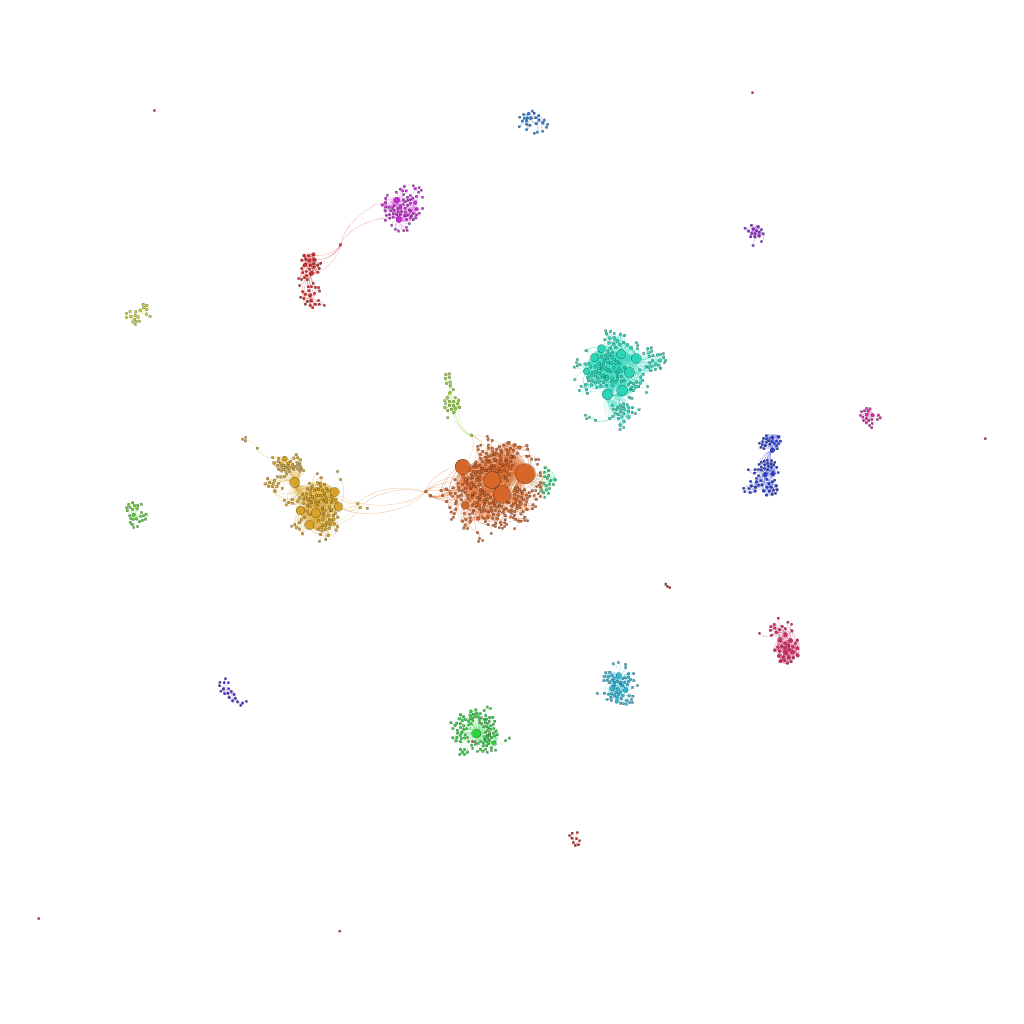
\includegraphics[width=6.0114in,height=6.0114in]{figures/chap3/chapitre3-img19.png}
    \caption{ {\textquotedblleft}Piaowudong nuzui{\textquotedblright}}
\end{figure}

Cet exemple présente les caractéristiques d{\textquoteright}une conversation très décentralisée dans laquelle de nombreux acteurs différents prennent part. L{\textquoteright}émergence de ce type de discussion fragmentée témoigne d{\textquoteright}un usage particulier de la discussion sur le réseau social et montre comment la discussion autour d{\textquoteright}un sujet peut s{\textquoteright}étendre sans afficher de relations directes dans le média lui-m\^eme. Ici un agent extérieur (en l{\textquoteright}occurence un article du journal \textit{Nanfang Zhoumo }sur le sujet) fait na\^itre la conversation sans pour autant l{\textquoteright}accaparer et la centraliser. Plus difficilement détectable et contr\^olable, cette dernière configuration est typique du mème car elle se développe de fa\c{c}on large et durable entre des groupes à l{\textquoteright}origine peu connectés.

Cette première visualisation des graphes conversationnels nous permet d{\textquoteright}explorer quelques types précis d{\textquoteright}échanges et d{\textquoteright}en proposer une première lecture. Néanmoins, le procédé de visualisation reste rudimentaire et soulève plusieurs questions que nous nous donnons pour t\^ache de continuer à explorer. Premièrement, dans quel espace a lieu cette représentation? En étalant ainsi ces graphes conversationnels, quelle action réalisons-nous réellement et quelle en est la valeur pour l{\textquoteright}analyse? à plus forte raison, quelle est la relation de cette espace du graphe conversationnel avec les autres formes d{\textquoteright}espace, et plus notamment l{\textquoteright}espace du réel géographique et l{\textquoteright}espace de la représentation par le langage?

\section{Méthodologie de traitement et de visualisation des mèmes}

L{\textquoteright}étude des relations entre ces différents types
d{\textquoteright}espaces implique donc une méthodologie renouvelée
et le développement d{\textquoteright}outils adaptés. Il ne
s{\textquoteright}agit plus simplement d{\textquoteright}étudier un
réseau, mais plus précisément de s{\textquoteright}interroger sur
les relations entre différents réseaux, de nature souvent
différentes. Au-delà du réseau multi-calques, nous sommes en
présence de multiples réseaux possédant des relations communes.

Nous avons donc sélectionné trois aspects importants des mèmes que
nous allons tenter de représenter au mieux afin d{\textquoteright}en
comprendre l{\textquoteright}existence :

\textbf{{}- }\textbf{\textit{langagier }}\textbf{:} le champ
sémantique d{\textquoteright}un mème est constitué des mots qui
sont prononcés lors de sa diffusion. L{\textquoteright}association de
mots -souvent sous la forme du jeu de mots - est un des propres du
mème et constitue ainsi une part importante de son existence. Ainsi,
le mème produit à proprement parler des réseaux de mots en
dessinant des liens entre des signifiants souvent improbables qui en
font souvent le succès \citep{Bauckhage2011}.

\textbf{\textit{{}- conversationnel }}\textit{: }au-delà des mots, un
mème se constitue sous la forme d{\textquoteright}un échange, une
conversation o\`u les différents acteurs discutent, commentent et se
saisissent des actions disponibles sur la pateforme web (like,
retweets, etc.) pour converser. Comme nous l{\textquoteright}avons vu
précédemment, nous pouvons identifier et considérer un graphe
conversationnel créé par le mème en se diffusant.

\textbf{\textit{{}- réel : }}au-delà des échanges en ligne, ces
discussions possèdent une existence physique, premièrement sous la
forme de l{\textquoteright}activité électrique des machines qui
sont utilisées lors de ce processus. Néanmoins, dans
l{\textquoteright}approche d{\textquoteright}une géographie humaine
des échanges numériques, nous considérerons ici
l{\textquoteright}existence physique des mèmes par celle des
utilisateurs - de leurs corps - et non pas des machines.

Afin d{\textquoteright}étudier chacun de ces aspects du mème, nous
allons donc procéder à la collection et la visualisation de
données sur chacun de ces niveaux d{\textquoteright}après un corpus
de mèmes sélectionnés.

\subsection[Sélection de mèmes pour l{\textquoteright}étude]{\textmd{\textup{ Sélection de
mèmes pour l{\textquoteright}étude}}}
Choisir un ensemble de mèmes cohérents est une des étapes
difficiles de notre recherche. En effet, dans le vaste corpus de
données utilisées et plus généralement dans la multitude des
échanges quotidiens sur les réseaux sociaux, trouver une prise pour
l{\textquoteright}étude n{\textquoteright}est pas une t\^ache
évidente. Afin de procéder à la sélection de mèmes, nous
avons donc choisi d{\textquoteright}utiliser la typologie des
catégories de mèmes identifiées dans la littérature (voir
partie 2) et d{\textquoteright}en systématiser
l{\textquoteright}usage sur notre corpus. Ainsi, pour chaque
catégorie, nous avons effectué une recherche m\^elant des sources
parlant des mèmes et de l{\textquoteright}Internet chinois (journaux,
blogs, encyclopédies en ligne, sites ressources), notre propre
expérience du web chinois et notre corpus de données disponibles.

Dans un premier temps, nous avons donc identifié pour chaque
catégorie de mème plusieurs évènements web de
l{\textquoteright}année 2012 sur Sina Weibo comme autant de candidats
pour représenter l{\textquoteright}ensemble de notre typologie. La
classification de l{\textquoteright}importance des évènements web
rev\^et une nature très différente selon les différentes sources.
Une revue de la littérature web sur les
{\textquotedblleft}évènements marquant du web social en
2012{\textquotedblright} montre que les contenus à caractère
politique et polémique sont considérés comme plus importants sur
les sites à audience majoritairement occidentale\footnote{ Global
Voices,
\ \ \ \url{http://globalvoicesonline.org/2012/12/07/top-10-chinese-internet-memes-of-2012/,}
consulté le 22 Avril 2014 à 12:10 ou WSJ
http://blogs.wsj.com/chinarealtime/2012/12/19/the-top-10-chinese-internet-memes-of-2012/,
consulté le 22 Avril 2014 à 12:10 } alors que les sites plus
spécialisés sur la Chine\footnote{ Danwei
\ \url{http://www.danwei.com/chinas-hottest-styles-of-2012/}
\ consulté le 22 Avril 2014 à 12:12} prennent davantage en
considération les phénomènes médiatiques commerciaux. Encore
une fois, nous voyons comment les réseaux sociaux chinois sont
représentés comme des phénomènes politiques, parfois au
détriment de leur existence comme média à part entière. Après
avoir comparé ces sources diverses, il nous fallait \^etre s\^ur que
nous disposions d{\textquoteright}une quantité suffisante de
données pour traiter le mème choisi. Nous avons donc indexé les
parties du corpus représentatives des différents évènements
afin de pouvoir effectuer des \ recherches plein-texte et ainsi
vérifier le volume et la qualité des corpus mobilisables pour
chaque mème. Pour ce faire, nous avons mis en place un outil
d{\textquoteright}indexation et de recherche\footnote{ Les technologies
utilisées pour indexer le corpus sont \textit{ElasticSearch }pour le
moteur de recherche et \textit{Kibana} pour le tableau de bord.
\url{http://www.elasticsearch.org} consulté le 22 Avril 2014 à
12:23} qui nous permet de contr\^oler les différents paramètres et
nous assurer de la quantité (taille significative), des dimensions
(dates correctes) et de la qualité du corpus (vérification du
contenu d{\textquoteright}un échantillon de 100 messages
sélectionnés aléatoirement).


\begin{figure}[th]
    \centering
    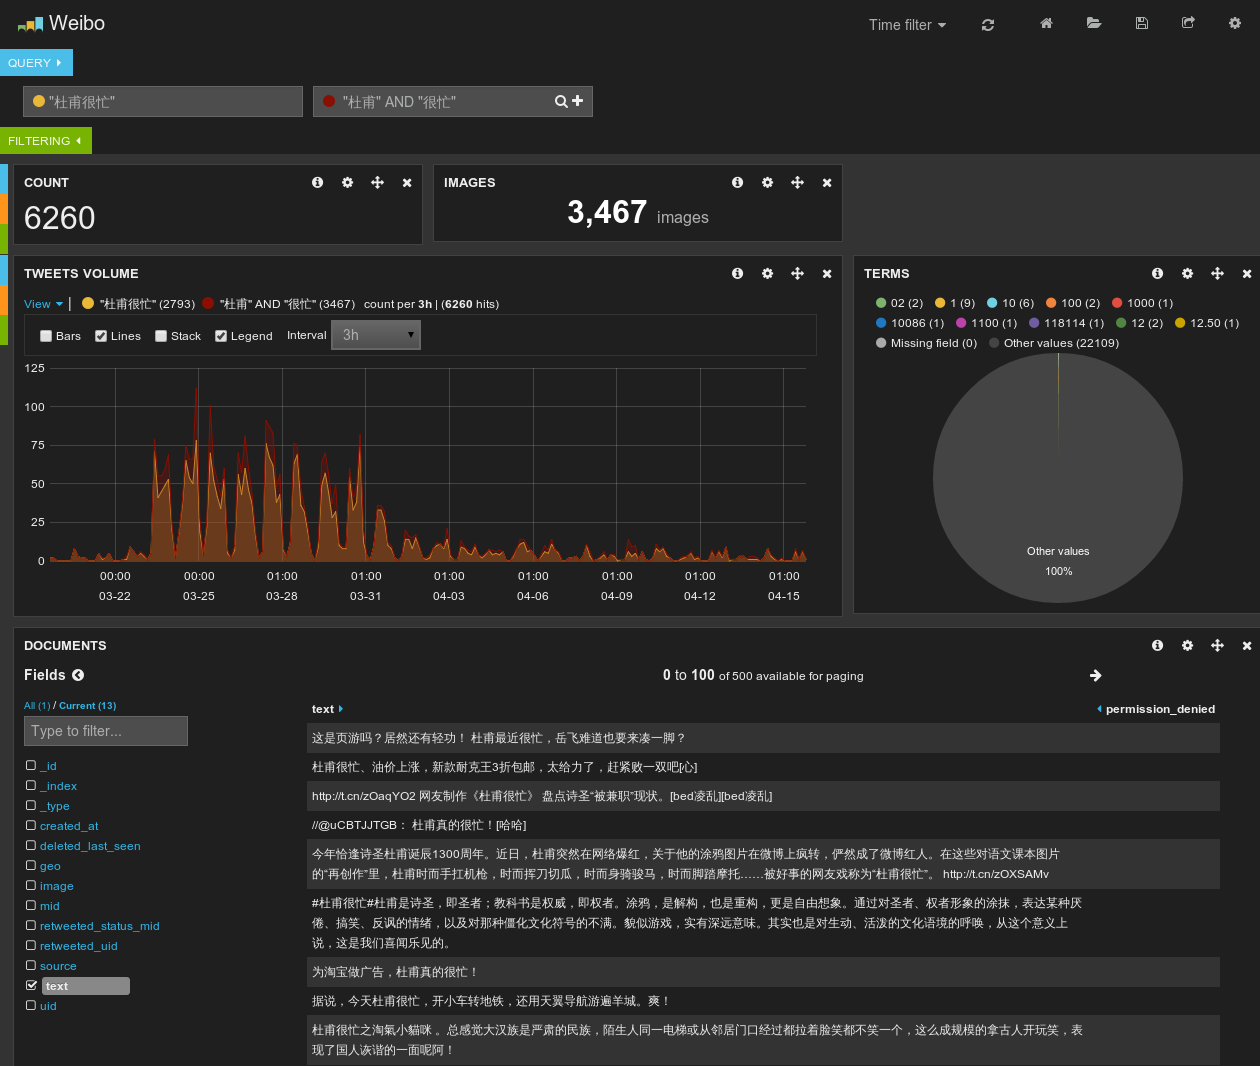
\includegraphics[width=6.0004in,height=5.078in]{figures/chap3/chapitre3-img20.png}
    \caption[Tableau de bords requêtes par mots-clés] { Ce tableau de bord permet de comparer la qualité de différentes requ\^etes dans le corpus. Capture d'écran réalisée le 23 Mars 2014 à 16h18}
\end{figure}


Cette étape nous a également permis d{\textquoteright}identifier les
mots-clés les plus appropriés pour définir chaque mème. En
effet, la qualité des archives pour chaque mème dépend fortement
de la méthode utilisée pour collecter les données. Ici, nous
utilisons la recherche plein texte pour collecter les données et nous
devons ainsi nous assurer que notre requ\^ete est bien construite, afin
de minimiser le bruit dans chaque corpus (éviter les messages
contenant les m\^eme mots-clés mais sans relations avec le mème). 

Une fois assuré qu{\textquoteright}un mème pouvait \^etre
correctement représenté dans un corpus de données, nous obtenons
donc une liste réduite de mèmes à étudier pour chaque
catégorie.

\begin{landscape}
\begin{table}

    \begin{tabulary}{\linewidth}{ r| C C C}

        \textbf{Début} & 
        \textbf{Nom} &  
        \textbf{Type} &  
        \textbf{Mots-Clés} \\

        \hline \\[-1.2ex]
        February 3, 2012 & 
        Campagne contre les touristes chinois à HK & 
        Actualité, satire, commentaire social &
        \zh{蝗蟲天下,蝗虫天下} \\

        March 21, 2012 &
        Détournement calligraphie : “Du Fu is very busy" &
        Absurdiste, humour &
        \zh{杜甫很忙,李白不服气了} \\

        April 22, 2012 &
        Chen Guancheng s'évade et se réfugie à l'ambassade des US &
        Marketing politique, soutien, pétition &
        \zh{陈光诚} \\

        May 30, 2012 & 
        Rumeur d'un coup d'état des proches de Boxilai (commentaires bloqués) &
        Marketing politique, soutien, pétition & 
        \zh{薄熙来,Zhou Yongkang} \\

        July 13, 2012 &  
        The Voice : lancement de l'émission TV &
         Fan clubs, adoration & 
        \zh{中国好声音, 吴莫愁} \\

        July 15, 2012 &  
        Gangnam Style : lancement du clip &  
        Fan clubs, adoration  &  
        \zh{鸟叔,江南STYLE} \\

        August 26, 2012 &
        Yang Dacai, l'officiel "souriant" et le scandale des montres &   
        Actualité, satire, commentaire social &  
        \zh{表叔,表哥,微笑局长,杨达才} \\

        September 21, 2012 & 
        Sortie du iPhone5   &
        Publicité, marketing viral & 
        \zh{iPhone, 苹果, Apple} \\

        October 1, 2012 & 
        Blague : "Yuan Fang, qu'est-ce que tu en penses?"  & 
        Absurdiste, humour & 
        \zh{远芳,你怎么看?,我觉得此事有蹊跷,神探狄仁杰} \\

        October 1, 2012 &
        Série TV : The Emperor's Harem & 
        Publicité, marketing viral &
        \zh{后宫,回家的诱惑,宫 (宫锁心玉)} \\

        October 11, 2012  &
        Mo Yan reçoit le Prix Nobel de littérature &
        Fan clubs, adoration  &
        \zh{莫言,管谟业,2012诺贝尔文学奖,诺贝尔} \\

        October 25, 2012 &
        Ai Weiwei sort son clip "Caonima style"&
        Actualité, satire, commentaire social &
        \zh{草泥马style, 艾虎子}\\

        November 8, 2012 &
        18ème Congrès du Parti Communiste &
        Marketing politique, soutien, pétition &
        \zh{第十八次全国代表大会,中共十八大,18大,十八大}\\

        November 20, 2012 &
        La sex tape de Lei Zhengfu publiée par un journaliste &
        Actualité, satire, commentaire social &
        \zh{雷政富}\\

        December 3, 2012  &
        Qiegao : échauffourées autour d'un gâteau du Xinjiang &
        Actualité, satire, commentaire social &
        \zh{切糕}\\

    \end{tabulary}
    % \caption[Liste d{\textquoteright}évènements web importants pendant l{\textquoteright}année 2012] 
\end{table}
\end{landscape}

\subsection{Extraction des graphes et traitement des données brutes}
Une fois cette requ\^ete clairement identifiée nous procédons pour
chaque mème à l{\textquoteright}extraction d{\textquoteright}un jeu
de données contenant l{\textquoteright}ensemble des messages
correspondant à la requ\^ete définie. Ce jeu de données est
ensuite complété par l{\textquoteright}ensemble des messages
mentionnés mais ne contenant pas le mot clé (commentaires,
réponses, etc.) afin d{\textquoteright}obtenir un ensemble de
messages représentatifs pour chaque mème.

Nous procédons ensuite au traitement de chaque corpus selon une
série de procédures définies comme suit :

\subsubsection{Graphe langagière (langagier ?)}

Le texte de chaque message est analysé de fa\c{c}on à ne conserver
que les mots les plus importants. Cela s{\textquoteright}effectue en
cinq étapes successives : 

\begin{enumerate}
\item La phrase est segmentée (analyse de la langue chinoise) pour
obtenir un ensemble de mots du mème.
\item A chacun des mots est associé l{\textquoteright}ensemble des
utilisateurs l{\textquoteright}ayant mentionné.
\item Les mots les plus courants sont enlevés afin de réduire le
bruit. La constitution de la liste des mots courants
\textit{(stopwords) }est une étape très importante. La liste que
nous utilisons a été créée à partir de différents corpus
lors d{\textquoteright}expérimentations précédentes et
augmentée de nouveaux mots au fur et à mesure.
\item La co-occurence d{\textquoteright}un mot dans une m\^eme phrase
définit une relation entre ces deux mots.
\item Parmi l{\textquoteright}ensemble de mots-clés ainsi obtenu, nous
conservons les 500 mots les plus utilisés (dont les occurences sont
les plus nombreuses) 
\item Nous reconstituons le graphe des relations entre ces 500
mots-clés d{\textquoteright}après la série de leur co-occurence :
chaque mot est un node, chaque co-occurence est un edge.
\item L{\textquoteright}ensemble constitue le graphe sémantique du
mème, pondéré mais non dirigé.
\end{enumerate}
\textbf{3.4.2.2. Graphe conversationnel}

Pour chaque mème, l{\textquoteright}ensemble des interactions
(mentions, citations et retweets) consituent le graphe conversationnel
o\`u un utilisateur est un node et une interaction est un edge. Le
graphe est dirigé car les interactions vont depuis un utilisateur à
un autre. 

Une fois l{\textquoteright}ensemble du graphe constitué, nous
déterminons sa modularité et son coefficient moyen de clustering
afin de posséder des informations sur sa structure. Nous calculons
également la centralité intermédiaire (\textit{betweenness
centrality}) pour chaque utilisateur dans l{\textquoteright}ensemble du
graphe. Ensuite, nous identifions les différentes communautés en
utilisant l{\textquoteright}algorithme dit de Louvain et son
implémentation par Blondel \& al. \citep{Blondel2008}\footnote{
\url{http://perso.crans.org/aynaud/communities/index.html} consulté
le 22 Avril 2014 à 14:24} qui nous permet d{\textquoteright}attribuer
à chaque utilisateur un groupe unique. Enfin, nous réduisons la
taille du graphe final en ne conservant que les utilisateurs ayant
effectué au moins 2 échanges - en supprimant les \textit{edges} du
graphe ayant un poids inférieur à 2.

Le graphe ainsi constitué correspond aux données conversationnelles
du mème.

\subsubsection{Localisation des utilisateurs}

Pour chaque mème, nous souhaitons également regrouper les
informations de localisation des utilisateurs mentionnés ou actifs
dans le mème. Le jeu de données \textit{Weiboscope }comprend les
localités mentionnées par les utilisateurs dans leurs profils. Le
nombre de ces localités est restreinte par
l{\textquoteright}interface de Sina Weibo elle-m\^eme à :
l{\textquoteright}ensemble des provinces de Chine continentale, Hong
Kong, Macau, Taiwan, {\textquotedblleft}à
l{\textquoteright}étranger{\textquotedblright} et
{\textquotedblleft}autres{\textquotedblright}. Ainsi, pour chaque
utilisateur nous assignons l{\textquoteright}information géographique
mentionnée par l{\textquoteright}utilisateur dans son profil.

\subsection{Visualisation multi-graphes}
Une fois que l{\textquoteright}ensemble de ces données a été
extrait et traité, nous pouvons considérer différents aspects au
sein du mème :

ii
\begin{description}
\item[Graphe sémantique] mots-clés et relations entre les mots
\item[Graphe socio-sémantique] relations entre les mots et les
utilisateurs
\item[Graphe conversationnel] relations et communautés
d{\textquoteright}utilisateurs 
\item[Graphe socio-géographique] relations entre les utilisateurs et
les provinces / villes chinoises
\end{description}

Nous avons donc plusieurs niveaux de lecture interdépendants qui nous
permettent de considérer différents aspects de chaque mème.
Néanmoins, les informations de graphe sont peu claires et
difficilement exploitables sous forme de données, à
l{\textquoteright}exception d{\textquoteright}une série de mesures
indicatives sur leurs structures. Afin d{\textquoteright}explorer ces
différentes relations, il nous faut pouvoir visualiser différentes
dimensions du mème afin d{\textquoteright}observer les articulations
et phénomènes possibles émergents de cette lecture. 

Pour réaliser cette cartographie particulière, il
n{\textquoteright}existe pas d{\textquoteright}outils disponibles
permettant de mettre en relation différents types de réseaux. Nous
avons donc choisi de développer une solution technologique adaptée
à nos besoins permettant de considérer sous différents angles
l{\textquoteright}ensemble de ces graphes et de leurs relations. Les
différents choix conceptuels et technologiques présidant au design
de cet outil de visualisation sont détaillés ci-après.

\subsubsection{Choix technologiques}

Les choix technologiques effectués lors de toute cette recherche et
plus particulièrement pour cet outil de visualisation ont vocation
à faciliter l{\textquoteright}interopérabilité et la publication
des résultats (visualisation, code et données) en ligne. Egalement,
l{\textquoteright}ensemble de l{\textquoteright}outil de visualisation
se fonde sur HTML5, CSS3 et Javascript qui sont des langages ouverts
issues d{\textquoteright}un travail collectif de
l{\textquoteright}ingénierie du Web permettant la réutilisation
partielle ou totale des travaux produits par d{\textquoteright}autres
et contribuant ainsi à davantage
d{\textquoteright}interopérabilité entre les différents design
scientifiques de recherche. La mise en forme des données utilise la
librairie {\textquotedblleft}Data-Driven Documents{\textquotedblright}
(d3.js)\footnote{ D3js at \url{http://d3js.org/,} consulté le 24
Avril 2014 à 14:58}, les données elles-m\^emes sont stockées en
JSON pour les graphes et GeoJSON pour les données cartographiques.

\subsubsection{Espace perceptif, plan projectif et choix
d{\textquoteright}un {\textquotedblleft}layout{\textquotedblright}}

Devant la disparité des données en présence, nous devons donc
construire un espace de représentation ou plut\^ot une interface de
représentation propice à l{\textquoteright}exploration et la
découverte des phénomènes dans les relations entre les
différents graphes. Dans la définition de cet espace perceptif se
joue la réconciliation d{\textquoteright}entités dissemblables (des
utilisateurs, des lieux, des mots, leurs relations mutuelles). La
t\^ache consisterait ainsi à réconcilier dans le plan de
l{\textquoteright}espace graphique de la visualisation (ici celui de
l{\textquoteright}écran) les différents espaces o\`u projeter ces
différents graphes. A l{\textquoteright}image du milieu numérique,
l{\textquoteright}existence m\^eme de ce plan réconciliant global,
local, réel, symbolique et imaginaire pose question. A la simple
question : {\textquotedblleft}quelle doit \^etre sa
couleur?{\textquotedblright}, une logique commune de lisibilité
répondrait : {\textquotedblleft}blanc ou noir{\textquotedblright},
mais quelle peut en \^etre la justification logique dans
l{\textquoteright}espace de la visualisation? Et que penser du coté
de l{\textquoteright}écran? De quoi est-t-il le bord? Dès lors que
se pose la question de structurer un espace de perception, nous voilà
devant plusieurs difficultés formelles majeures.
L{\textquoteright}exigence de rigueur scientifique et surtout
l{\textquoteright}imperméabilité des formats de publications
scientifiques actuelles rajoutent à la compexité de cette
entreprise.

Afin de pouvoir considérer les relations entres mots, communautés et
territoires, nous devons dans l{\textquoteright}espace graphique
disponible, il est nécessaire de résoudre plusieurs problèmes :

ii
\begin{itemize}
\item Donner à voir chaque type d{\textquoteright}entités de
fa\c{c}on reconnaissable (provinces chinoises, communautés, mots)
\item Donner à voir les relations entre les différentes entités
(graphe multiples)
\item Pallier l{\textquoteright}augmentation de la complexité visuelle
et préserver une lisibilité
\end{itemize}
Nous avons donc choisi de construire un espace sur plusieurs niveaux
hiérachisés.

\subsubsection{Graphes et interactions}

Le centre de la visualisation est occupé par les utilisateurs,
reflétant à la fois l{\textquoteright}intér\^et central de cette
étude pour l{\textquoteright}étude des processus
d{\textquoteright}individuation et le r\^ole charnière des
utilisateurs dans la structuration des données. Plus exactement, nous
avons choisi de regrouper les utilisateurs par communautés afin de
considérer les liens qui les unissaient entre elles et la structure
générale de la discussion plut\^ot que de
s{\textquoteright}intéresser aux individus. Les individus sont
symbolisés par des points au sein des communautés dont la couleur
indique leur centralité dans le réseau global. 

Notre première idée a été de représenter
l{\textquoteright}ensemble des utilisateurs sur une carte pour
comprendre comment s{\textquoteright}agencaient spatialement chacune
des discussions. La première étape a donc été de reconstituer
une carte de la Chine comprenant Taiwan, Hong Kong et Macau. Chacun de
ces territoires possèdent une influence médiatique certaine en
Chine et méritent à ce titre d{\textquoteright}\^etre
représenté. Néanmoins, le statut politique particulier de chacun
de ces territoires nous a obligé à reconstituer une carte o\`u ils
figuraient tous. Nous avons choisi d{\textquoteright}aggrandir
l{\textquoteright}échelle de Hong Kong et Macau afin
qu{\textquoteright}il soit visible sur la carte. Egalement, nous avons
choisi de ne pas restituer les données concernant les utilisateurs
ayant choisi {\textquotedblleft}autres{\textquotedblright} ou
{\textquotedblleft}reste du monde{\textquotedblright} comme leurs lieux
de résidence.

Si la carte se pr\^ete assez bien à la visualisation de quantité,
les visualisations de graphe deviennent facilement confuses. Ainsi,
nous avons choisi d{\textquoteright}ajouter une option de visualisation
des provinces sous la forme d{\textquoteright}une liste, au moins toute
aussi parlante. Cela nous permet en plus d{\textquoteright}organiser
cette liste selon différents critères afin
d{\textquoteright}étudier plusieurs aspects qui peuvent \^etre
intéressants.

Le graphe de mots rev\^et ici la forme la plus simple. Les relations
entre les mots sont matérialisées par un graphe utilisant un
algorihme force-based pour disposer les mots entre eux, recréant
ainsi des groupes de mots intéressants d{\textquoteright}après leur
proximité dans les phrases lors des discussions. Un positionnement
des mots selon leur importance (nombre de citations) est également
disponible à loisir.

Afin d{\textquoteright}explorer les différentes dimensions du graphes,
nous avons également ajouté des interactions qui permettent de
focaliser sur des zones ou des caractéristiques précises des
graphes. \citep{Bostock2011}

\begin{figure}
    \centering
    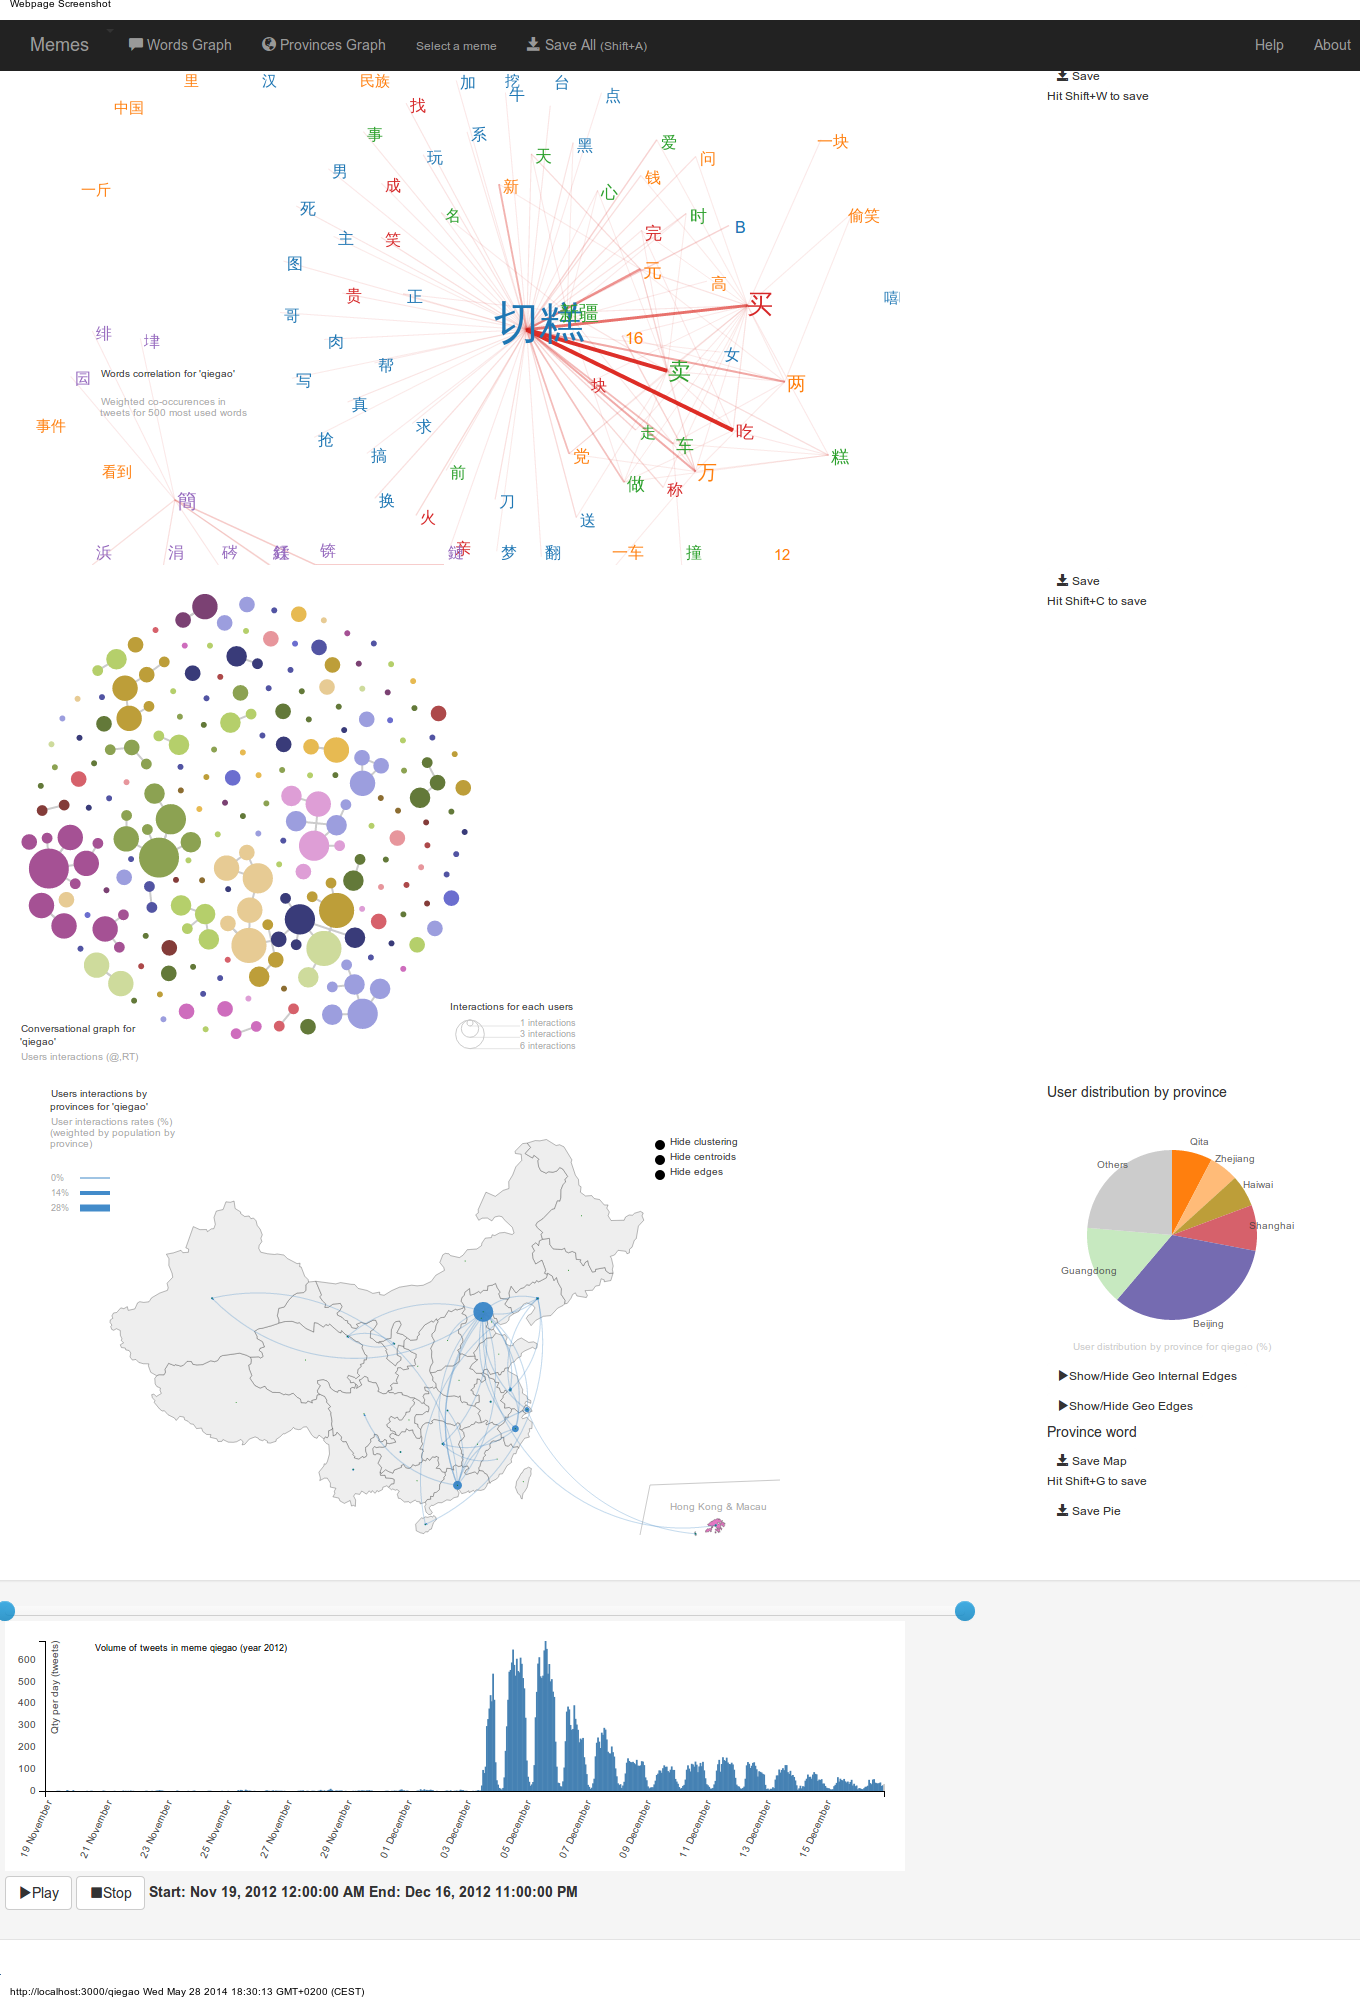
\includegraphics[width=6.7213in,height=8.3894in]{figures/chap3/chapitre3-img21.png}
    \caption{Interface d'exploration et de visualisation des données}
\end{figure}